\appendix

\chapter{M\lowercase{athematical} B\lowercase{ackground}}


\section{Gaussian Identities} \label{app:gauss}
This section follows closely Appendix A.2 in \cite{RaWi06}. The multivariate Gaussian distribution over the random vector space $\bx \in \RR^D$ has a probability density given by
\begin{equation}
\cN\bil\bx|\bm,\bS\bir = (2\pi)^{-D/2} |\bS|^{-1/2} \exp \bil -\half (\bx - \bm)\T\bS\inv (\bx - \bm) \bir
\end{equation}
where $\bm \in \RR^D$ is the mean and $\bS\in \RR^{D\times D}$ is the covariance. Let $\bx$ and $\by$ be jointly Gaussian random vectors
\begin{equation}
\bmat{\bx \\ \by} \sim \cN\left(
\bmat{\bm_{\bx} \\ \bm_{\by}},
\bmat{\bS_{\bx} & \bS_{\bx\by} \\ \bS_{\bx\by}\T & \bS_{\by}}
\right)
\end{equation}
then the \textit{marginal} distribution of $\bx$ and the \textit{conditional} distribution of $\bx$ given $\by$ are
\begin{align}
\bx &\sim \cN\big( \bm_{\bx}, \bS_{\bx} \big) \\
\bx|\by &\sim \cN\big( \bm_{\bx} + \bS_{\bx\by} \bS_{\by}^{-1} \big( \by - \bm_{\by} \big),
\bS_{\bx} - \bS_{\bx\by} \bS_{\by}^{-1} \bS_{\bx\by}\T \big)
\end{align}
The product of two Gaussians gives another (unnormalised) Gaussian
\begin{align}
\cN(\bx|\ba, \bA)\cN(\bx|\bb, \bB) &= c^{-1}\cN\big(\bx|\bc, \bC \big) 
\end{align}
where the normalising constant is itself a Gaussian $c^{-1} = \cN(\ba|\bb, \bA+\bB)$ and the mean and covariance are given by
\begin{align*}
\bc &= (\bA^{-1} + \bB^{-1})^{-1}(\bA^{-1}\ba + \bB^{-1}\bb)
&&\!\!\!\!\!\!\!\!\!\!\!\!\!\!\!\!\!\!\!\!\!\!\!\!\!\!\!\!\!\!\! = \bB(\bA + \bB)^{-1}\ba + \bA(\bA + \bB)^{-1}\bb \\
\bC &= (\bA^{-1} + \bB^{-1})^{-1}
&&\!\!\!\!\!\!\!\!\!\!\!\!\!\!\!\!\!\!\!\!\!\!\!\!\!\!\!\!\!\!\! = \bB(\bA + \bB)^{-1}\bA
\end{align*}
To generate samples from a multivariate Gaussian distribution $\bx \sim \cN(\bm,\bS)$ using a scalar Gaussian generator, first compute the Cholesky decomposition $\bL$ of the covariance matrix $\bS = \bL\bL\T$ where $\bL$ is lower triangular. Next, generate a random vector $\bu \sim \cN(\mathbf{0}, \bI)$ using independent scalar samples. Compute $\bx = \bm + \bL\bu$ which has the desired distribution with expectation $\EE[\bx] = \bm + \bL\EE[\bu] = \bm$ and covariance $\cov[\bx] = \bL\cov[\bu]\bL\T = \bL\bL\T = \bS$.



\section{Kullback-Leibler Divergence} \label{app:KLdiv}
This section is taken from Appendix A.5 in \cite{RaWi06}. The Kullback-Leibler (KL) divergence $\mathrm{KL}(p || q)$ of some distribution $p(\bx)$ with respect to $q(\bx)$ is defined as
\begin{equation}
\mathrm{KL}(p || q) = \int p(\bx) \log \frac{p(\bx)}{q(\bx)} \dd\bx
\end{equation}
The KL divergence of a distribution $p(\bx)$ on $\RR^D$ with respect to some Gaussian distribution $q(\bx) = \cN(\bm,\bS)$ is
\begin{align}
\mathrm{KL}(p || q) &= \int \Big( \half(\bx - \bm)\T\bS\inv (\bx - \bm) + \log\big(p(\bx)\big) \Big) p(\bx) \dd\bx 
+ \half\log|\bS| + \tfrac{D}{2}\log 2\pi
\end{align}
This can be minimised with respect to $\bm$ and $\bS$ by differentiating with respect to these parameters and setting the resulting expression to zero. It turns out the the optimal $q$ is the one with first moment $\int\bx p(\bx)\dd\bx$ and second moment $\int\bx\bx\T p(\bx)\dd\bx$ i.e.\ the moment matched solution.




\section{Matrix Calculus} \label{app:matcal}
The convention for dealing with derivatives of matrices with respect to matrices is taken from \cite{Bro05} which makes use of the vectorisation operation to ensure that all algebra remains in terms of standard matrix operations.
Consider the matrices $\bX \in \RR^{m\times n}$ and $\bY \in \RR^{p\times q}$ then the derivative of $\bY$ with respect to $\bX$ could be viewed in terms of a fourth-order tensor $\dpp\bY/\dpp\bX \in \RR^{p\times q \times m\times n}$. However, these are awkward to deal with computationally so define the derivative as follows
\begin{equation}
\pdiff{\bY}{\bX} := \pdiff{\vect(\bY)}{\vect(\bX)} = 
\begin{bmatrix}
\pdiff{\bY[:,1]}{\bX[:,1]} & \dots & \pdiff{\bY[:,1]}{\bX[:,n]} \\
\vdots & \ddots & \vdots \\
\pdiff{\bY[:,q]}{\bX[:,1]} & \dots & \pdiff{\bY[:,q]}{\bX[:,n]}
\end{bmatrix}
\in \RR^{pq \times mn}
\label{eqn:dvecdvec}
\end{equation}
consisting of blocks $\partial\bY[:,i]/\partial\bX[:,j] \in \RR^{p\times m}$. This convention will also hold for vectors and scalars (for which the $\vect$ operation has no effect). For example, for scalars $y$ and $x$ and vectors $\by \in \RR^p$ and $\bx \in \RR^m$ the dimensions of the associated derivatives are as follows with elements determined by the definition in \Eq{dvecdvec}
\begin{align*}
\pdiff{y}{x} &\in \RR &
\pdiff{y}{\bx} &\in \RR^{1\times m} &
\pdiff{y}{\bX} &\in \RR^{1\times mn}
\\[0.1cm]
\pdiff{\by}{x} &\in \RR^{p} &
\pdiff{\by}{\bx} &\in \RR^{p\times m} &
\pdiff{\by}{\bX} &\in \RR^{p\times mn}
\\[0.1cm]
\pdiff{\bY}{x} &\in \RR^{pq} &
\pdiff{\bY}{\bx} &\in \RR^{pq\times m} &
\pdiff{\bY}{\bX} &\in \RR^{pq\times mn}
\end{align*}

Now consider a third matrix $\bZ \in \RR^{q\times r}$ which is dependent on $\bX$ through $\bY$. The chain rule and product rule can be written as
\begin{align}
&\text{\it Chain Rule: } & 
\!\!\!\!\!\!\!\!\!\!\!\!\!\!\!\!\!\!\!\!\!\!\!\!
\pdiff{\bZ}{\bX} &= \pdiff{\bZ}{\bY}\pdiff{\bY}{\bX} \\[0.2cm]
&\text{\it Product Rule: } & 
\!\!\!\!\!\!\!\!\!\!\!\!\!\!\!\!\!\!\!\!\!\!\!\!
\pdiff{(\bY\bZ)}{\bX} &= (\bI\otimes\bY)\pdiff{\bZ}{\bX} + (\bZ^\top\otimes\bI)\pdiff{\bY}{\bX}
\end{align}

Some further useful results where $\bA$, $\bB$ and $\bC$ are matrices independent of $\bX$ and of appropriate dimensions are
\begin{align}
\pdiff{}{\bX} \bil \bX\T \bir &= \bT_{m,n} \\
\pdiff{}{\bX} \bil \bA^\top\bX\bB \bir &= (\bB\otimes\bA)^\top \\
\pdiff{}{\bX} \bil \bX^\top\bC\bX \bir &= (\bI\otimes\bX^\top\bC) + (\bX^\top\bC^\top\otimes\bI)\bT_{m,n}
\end{align}
The matrix $\bT_{m,n} \in \RR^{mn \times mn}$ is the \textit{vectorised transpose matrix} whose $(i,j)^{\text{th}}$ element is equal to one if $j=1+m(i-1)-(mn-1)\lfloor(i-1)/n\rfloor$ and zero otherwise.





\chapter{E\lowercase{quations of} M\lowercase{otion}}


\section{Pendulum} \label{app:pend}
The pendulum system used in this thesis is shown in \Fig{pendfig}, along with the forces and moments that act on it. Resolving the rate of change of angular momentum around the pivot point gives
\begin{align}
\nonumber I\ddot\theta &= u - T_{\te{f}} - \tfrac{1}{2}l(W\sin\theta) \\
\tfrac{1}{3}ml^2 \ddot{\theta} &= u - b\dot\theta - \tfrac{1}{2}mlg\sin\theta
\end{align}
where we consider the pole to be of uniform density. The variables $I$, $T_{\te{f}}$ and $W$ refer to the moment of inertia (about the pivot point), friction torque and weight respectively. The constants we used were mass $m=1\,$kg, length $l=1\,$m, friction $b = 0.1\,$N$\,$s$\inv$ and gravitational acceleration $g=9.81\,$m$\,$s$^{-2}$. This system then has states $\bx = [\theta; \dot\theta]^\top$ and we constrain the input torque such that $u\in [-3,3]\,$N$\,$m.



%-------------------------------------------------------------------------------------------------------------------------------------------
\begin{figure}
\centering
\small
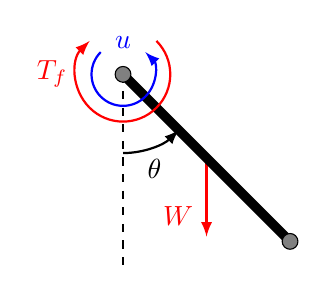
\begin{tikzpicture}[]
	\draw[-latex,thick,red] (1.0607,-1.0607) -- (1.0607,-2.0607); % 1.25/sqrt(2)
	\draw[line width=1.2mm, rotate=45] (0,0) -- (0,-3);
	\draw[dashed] (0,0) -- (0,-2.5);
	\draw[rotate=-90,-latex,thick] (1,0) arc (0:45:1cm);
	\draw[-latex,thick,blue] (-0.2828,0.2828) arc (-225:45:0.4cm); % 0.4/sqrt(2)
	\draw[-latex,thick,red] (0.4243,0.4243) arc (45:-225:0.6cm); % 0.6/sqrt(2)
	\draw[fill=gray] (0,0) circle (1mm);
	\draw[fill=gray,rotate=45] (0,-3) circle (1mm);
	
	\node[] at (0.4,-1.2) {$\theta$};
	\node[] at (0,0.4) {\color{blue} $u$};
	\node[] at (-0.9,0) {\color{red} $T_{\te{f}}$};
	\node[] at (0.7,-1.8) {\color{red} $W$};
\end{tikzpicture}
\caption{Torque-limited pendulum with angle from the down position $\theta$, input torque $u$, weight $W$ and friction torque $T_{\te{f}}$.}
\label{fig:pendfig}
\end{figure}
%-------------------------------------------------------------------------------------------------------------------------------------------






%-------------------------------------------------------------------------------------------------------------------------------------------
\begin{figure}
\centering
\small
\subfigure[Cart free body diagram]{
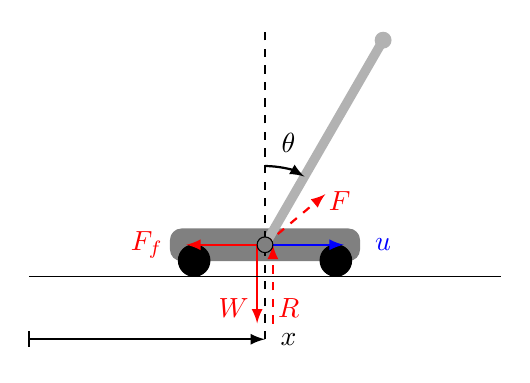
\begin{tikzpicture}[]
	
	\draw[fill=black!50, black!50, rounded corners] (-1.2,-0.2) rectangle (1.2,0.2); % body
	\draw[fill=black] (0.9,-0.2) circle (.2cm); \draw[fill=black] (-0.9,-0.2) circle (.2cm); % wheels
	\draw[black!30, line width = 1.2mm, rotate=-30] (0,0) -- (0,3); % pole
	
	\draw[-latex, blue, thick] (0, 0) -- (1,0);
	\draw[-latex, red, thick] (0, 0) -- (-1,0);
		
	\draw[dashed] (0,-1.2) -- (0,2.75);
	
	\draw[-latex, red, thick] (-0.1, 0) -- (-0.1,-1);
	\draw[-latex, red, dashed, thick] (0.1, -1) -- (0.1,0);
	\draw[red,dashed,-latex,thick,rotate=-50] (0,0) -- (0,1);
	
	\draw[rotate=90, -latex,thick] (1,0) arc (0:-30:1cm);
	\draw[fill=black!15, black!30] (1.5,2.5981) circle (1mm); 
	\draw[fill=gray] (0,0) circle (1mm);
	
	\node[] at (0.3,1.3) {$\theta$};
	
	\draw[] (-3,-0.4) -- (3,-0.4);
	
	\node[] at (0.3,-1.2) {$x$};
	\draw[thick] (-3, -1.1) -- (-3,-1.3);
	\draw[-latex,thick] (-3, -1.2) -- (0,-1.2);
	
	\node[] at (1.5,0) {\color{blue}$u$};
	\node[] at (-1.5,0) {\color{red}$F_{\te{f}}$};
	\node[] at (0.95,0.55) {\color{red}$F$};
	\node[] at (-0.4,-0.8) {\color{red}$W$};
	\node[] at (0.3,-0.8) {\color{red}$R$};

	
\end{tikzpicture}
\label{fig:pole_FBD}
}
\subfigure[Pole free body diagram]{
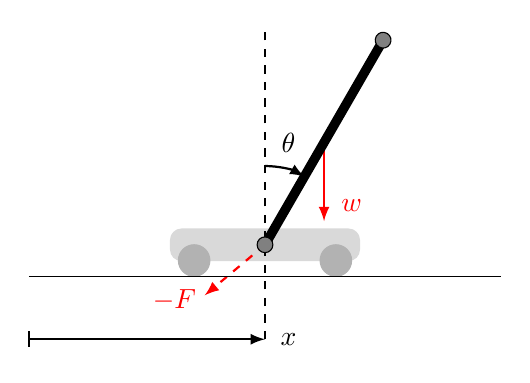
\begin{tikzpicture}[]
	
	
	\draw[fill=black!15, black!15, rounded corners] (-1.2,-0.2) rectangle (1.2,0.2); % body
	\draw[red,thick,-latex] (0.75,1.299) -- (0.75,0.299);
	\draw[fill=black!30,black!30] (0.9,-0.2) circle (.2cm); % wheels
	\draw[fill=black!30,black!30] (-0.9,-0.2) circle (.2cm);
	\draw[fill=black, line width = 1.2mm, rotate=-30] (0,0) -- (0,3); % pole
	
	\draw[dashed] (0,-1.2) -- (0,2.75);
	\draw[rotate=90, -latex,thick] (1,0) arc (0:-30:1cm);

	\draw[red,dashed,-latex,thick,rotate=-50] (0,0) -- (0,-1);
	\draw[fill=gray, rotate=-30] (0,3) circle (1mm);
	\draw[fill=gray] (0,0) circle (1mm);
	
	\node[] at (0.3,1.3) {$\theta$};
	\node[] at (1.1,0.5) {\color{red} $w$};
	\node[] at (-1.15,-0.7) {\color{red} $-F$};
	
	\draw[] (-3,-0.4) -- (3,-0.4);
	
	\node[] at (0.3,-1.2) {$x$};
	\draw[thick] (-3, -1.1) -- (-3,-1.3);
	\draw[-latex,thick] (-3, -1.2) -- (0,-1.2);

	
\end{tikzpicture}
\label{fig:cart_FBD}
}
\caption{Cart-pole free body diagrams with position $x$,  pole angle $\theta$, action force $u$, weight of the pole $w$, weight of the cart $W$, friction force $F_{\te{f}}$, internal force $F$ and reaction force $R$. }
\label{fig:cartpole_FBD}
\end{figure}
%-------------------------------------------------------------------------------------------------------------------------------------------




\section{Cart-Pole} \label{app:cart}
The cart-pole system used in this thesis is shown by the free body diagrams in \Fig{cartpole_FBD}, along with the forces and moments that act upon it. The following derivation is based on that of \cite{Flo07}. We shall begin by considering the free body diagram of the cart alone, shown in \Fig{cart_FBD}, and balancing the forces and accelerations in the lateral direction. Doing this we get
\begin{align}
M\ddot x &=  u - F_{\te{f}} + F_x
\label{eqn:cart1}
\end{align}
where $x$ is the lateral position of the cart, $\theta$ is the angle of the pole, $M$ is the mass of the cart, $F_x$ is the lateral component of the internal force between cart and pole, $u$ is the driving force and $F_{\te{f}}$ is the friction force. Now we turn to the free body diagram of the pole, shown in \Fig{pole_FBD}, and balance the forces and accelerations along the lateral and vertical directions. This yields
\begin{align}
m\big(\ddot x + \tfrac{1}{2}l\ddot\theta\cos\theta - \tfrac{1}{2}l\dot\theta^2\sin\theta\big) &= -F_x
\label{eqn:cart2} \\
m\big(\tfrac{1}{2}l\ddot\theta\sin\theta + \tfrac{1}{2}l\dot\theta^2\cos\theta\big) &= mg + F_y
\label{eqn:cart3}
\end{align}
respectively, where $m$ is the mass of the pole and $l$ is its length. The $\tfrac{1}{2}ml\dot\theta^2$ and $\tfrac{1}{2}ml\ddot\theta$ terms are the accelerations due to the angular acceleration of the pole, or the ``fictitious'' forces. Finally, if we balance the torques and angular accelarations around the joint we get
\begin{align}
I\ddot\theta + \tfrac{1}{2}m\ddot xl\cos\theta &= \tfrac{1}{2}mgl\sin\theta
\label{eqn:cart4}
\end{align}
with moment of intertia $I = \tfrac{1}{3}ml^2$ for a pole of uniform density.
We can now eliminate the components of the internal force, $F_x$ and $F_y$, to find the two equations of motion. Substitute \Eq{cart1} into \Eq{cart2} and rearrange \Eq{cart4} to yield the relationships
\begin{align}
(M+m)\ddot x &= \tfrac{1}{2}ml(\dot\theta^2\sin\theta - \ddot\theta\cos\theta) + u - b\dot x 
\label{eqn:cart5}\\
l\ddot\theta &= \tfrac{3}{2}g\sin\theta - \tfrac{3}{2}\ddot x\cos\theta
\label{eqn:cart6}
\end{align}
where we employ a linear friction model $F_\te{f} = b\dot x$. \Eqs{cart5}{cart6} can then be rearranged to isolate the terms $\ddot x$ and $\ddot\theta$ and give the equations of motion for this system.
The action force was constrained to $u \in [-10,10]\,$N and the physical constants we used were: length $l = 1\,$m, mass of cart $M = 0.5\,$kg, mass of pole $m = 0.5\,$kg and coefficient of friction $b = 0.1\,$N$\,$s$\,$m$\inv$. 

%The equations of motion governing this system for a pole of uniform density can be derived as
%\begin{align}
%\ddot x &= \frac{ m_{\te{p}} \big( 2 l \dot\theta^2 + 3g\cos\theta \big) \sin\theta  + 4(u - b\dot x) }{ 4(m_{\te{c}}+m_{\te{p}}) - 3m\cos^2\theta } \\
%\ddot \theta &= \frac{ -3 \big( m_{\te{p}} l \dot\theta^2\cos\theta + 2g(m_{\te{c}}+m_{\te{p}})\big) \sin\theta  -6(u - b\dot x)\cos\theta }{ l\big(4(m_{\te{c}}+m_{\te{p}}) - 3m\cos^2\theta\big) }
%\end{align}
%The state of this system $\bx = [x,\dot x, \theta, \dot\theta]$ consists of the position of the cart along the track $x\,$m, the angle of the pendulum from the upright $\theta$ and the associated velocity terms. The input is simply the lateral force applied to the cart $u\,$N.





%-------------------------------------------------------------------------------------------------------------------------------------------
\begin{figure}
\centering
%set the plot display orientation
%synatax: \tdplotsetdisplay{\theta_d}{\phi_d}
\tdplotsetmaincoords{65}{100}

%define polar coordinates for some vector
%TODO: look into using 3d spherical coordinate system
\pgfmathsetmacro{\magW}{4}
\pgfmathsetmacro{\psiW}{-30}
\pgfmathsetmacro{\theW}{10}
\pgfmathsetmacro{\phiW}{15}

%start tikz picture, and use the tdplot_main_coords style to implement the display 
%coordinate transformation provided by 3dplot
\footnotesize
\begin{tikzpicture}[scale=0.95,tdplot_main_coords]

%set up some coordinates ... GET FROM MATLAB
%-----------------------
\coordinate (O) at (1.7321,-1,0);
\coordinate (B) at (2.5,4.3301,0);
\coordinate (Bp) at (4.2321,3.3301,0);
\coordinate (W) at (2.7256,4.1999,1.4772);
\coordinate (Wt) at (3.1767,3.9394,4.4316);
\coordinate (Wtp) at (2.7256,4.1999,4.4316);
\coordinate (Wbp) at (2.7256,4.1999,0);
\coordinate (T) at (2.7969,2.8138,5.7578);
\coordinate (F) at (2.7612,3.5069,3.6175);

%draw figure contents
%--------------------

%draw the main coordinate system axes
\tdplotsetrotatedcoordsorigin{(O)}
\tdplotsetrotatedcoords{0}{0}{0}
\draw[tdplot_rotated_coords,-latex,blue,thick] (0,0,0) -- (1.5,0,0) node[anchor=south east]{$\bi$};
\draw[tdplot_rotated_coords,-latex,blue,thick] (0,0,0) -- (0,1.5,0) node[anchor=south]{$\bj$};
\draw[tdplot_rotated_coords,-latex,blue,thick] (0,0,0) -- (0,0,1.5) node[anchor=south]{$\bk$};
\draw[dashed] (W) -- (Wt);
\draw[dashed] (Wtp) -- (Wbp);
\draw[dashed] (B) -- (W);

\draw[red,-latex] (B) -- (Bp);
\draw[red,-latex] (Bp) -- (O);
\node at (0,0.8,-1.7) {\color{red} $x_\te{c}$};
\node at (0,3.2,-1.4) {\color{red} $y_\te{c}$};
\tdplotsetrotatedcoords{\psiW}{0}{0}
\tdplotsetrotatedcoordsorigin{(Bp)}
\draw[tdplot_rotated_coords,very thin] (-0.35,0,0) -- (-0.35,-0.35,0) -- (0,-0.35,0);


% draw frame
\draw[very thick,black] (W) -- (T);
\tdplotsetrotatedcoords{\psiW}{100}{0}
\tdplotsetrotatedcoordsorigin{(F)}
\draw[tdplot_rotated_coords,fill=black] (0,0,0) circle (0.12);

% draw turntable
\tdplotsetrotatedcoords{\psiW}{\theW}{\phiW}
\tdplotsetrotatedcoordsorigin{(T)}
\draw[tdplot_rotated_coords,very thick,fill=black,fill opacity=0.2] (0,0,0) circle (1.5);
\draw[tdplot_rotated_coords,fill=black] (0,0,0) circle (0.12);
\tdplotdrawarcarrow[tdplot_rotated_coords,red]{(T)}{0.65}{0}{270}{}{}
\tdplotdrawarcarrow[tdplot_rotated_coords,blue]{(T)}{0.4}{0}{270}{}{}
\node at (0,3.25,4.8) {\color{red} $\psi_\te{t}$};
\node at (0,1.7,4.2) {\color{blue} $u_\te{t}$};

% draw wheel
\tdplotsetrotatedcoords{\psiW}{100}{0} % add 90 to j angle
\tdplotsetrotatedcoordsorigin{(W)}
\draw[tdplot_rotated_coords,very thick,fill=black,fill opacity=0.2] (0,0,0) circle (1.5);
\draw[tdplot_rotated_coords,fill=black] (0,0,0) circle (0.12);
\tdplotdrawarcarrow[tdplot_rotated_coords,red]{(W)}{0.6}{0}{270}{}{}
\tdplotdrawarcarrow[tdplot_rotated_coords,blue]{(W)}{0.4}{0}{270}{}{}
\node at (0,4.35,0.5) {\color{red} $\phi_\te{w}$};
\node at (0,3.3,-0.1) {\color{blue} $u_\te{w}$};



% show theta and phi
\tdplotdrawarcarrow[red]{(O)}{0.8}{0}{60}{anchor=north}{\color{red} $\psi$}
\tdplotsetrotatedcoords{\psiW}{190}{-90} % add 180 to j angle
\tdplotsetrotatedcoordsorigin{(W)}
\tdplotdrawarcarrow[tdplot_rotated_coords,red]{(W)}{2.8}{80}{90}{anchor=south}{\color{red} $\theta$}
\tdplotsetrotatedcoords{\psiW}{100}{0} % add 90 to j angle
\tdplotsetrotatedcoordsorigin{(W)}
\tdplotdrawarcarrow[tdplot_rotated_coords,red]{(W)}{2.8}{180}{195}{anchor=south}{\color{red} $\phi$}


\end{tikzpicture}
\caption{The robotic unicycle with state variables: pitch angle $\phi$, roll angle $\theta$, yaw angle $\psi$, wheel angle $\phi_\te{w}$, turntable angle $\psi_\te{t}$, the associated angular velocities and the location of the global origin $(x_\te{c},y_\te{c})$. The actions are the wheel motor torque $u_\te{w}$ and the turntable motor torque $u_\te{t}$. The global coordinate system is defined by the vectors $\bi, \bj$ and $\bk$.}
\label{fig:unibody}
\end{figure}
%-------------------------------------------------------------------------------------------------------------------------------------------





\section{Unicycle} \label{app:unicycle}
\subsection{Method}
The robotic unicycle is shown in \Fig{unibody} with global coordinate system defined by the orthonormal vectors $\bi, \bj$ and $\bk$. The spatial position of the unicycle is fully defined by the pitch angle $\phi$, roll angle $\theta$, yaw angle $\psi$, wheel angle $\phi_\te{w}$, turntable angle $\psi_\te{t}$ and location of the global origin with respect to the body-centred coordinate system $(x_\te{c},y_\te{c})$. We chose the state vector to be $\bx = [\phi,\dot\phi,\theta,\dot\theta,\psi,\dot\psi,\dot\phi_\te{w},\dot\psi_\te{t},x_\te{c},y_\te{c}]\T \in\RR^{10}$ where we exclude $\phi_\te{w}$ and $\psi_\te{t}$ since they clearly have no effect on the dynamics. The action vector $\bu$ is made up of a wheel motor torque $u_\te{w}$ and a turntable motor torque $u_\te{t}$.
The equations of motion that govern the unicycle were derived by \cite{For09}. We shall provide a sketch of the full derivation here, in which we follow the steps taken by Forster in Section 3.3 of his thesis. 

Let us start with the coordinates $(x_\te{c},y_\te{c})$. These are centred on the point of contact with the floor and define the location of the global origin. The coordinate $x_\te{c}$ lies parallel to the current direction of travel and $y_\te{c}$ is orthogonal to it. These coordinates evolve according to
\begin{align}
\dot x_\te{c} &= r_\te{w} \dot\phi_\te{w} \cos\psi \label{eqn:xceqn}  \\
\dot y_\te{c} &= r_\te{w} \dot\phi_\te{w} \sin\psi \label{eqn:yceqn}
\end{align}
where $r_\te{w}$ is the wheel radius.
The full unicycle model was obtained by analysing the wheel, frame and turntable as individual Free Body Diagrams (FBDs), as depicted in \Fig{FBDs}. Linear momentum and moment of momentum for each FBD were then resolved to yield six scalar equations for each free body. The internal forces were then eliminated to yield five independent scalar equations which govern the evolution of the angular states. A description of the physical constants of the system along with the values we use in this thesis are given in \Tab{uniconsts}.





%-------------------------------------------------------------------------------------------------------------------------------------------
\begin{table}
\renewcommand{\arraystretch}{1.3}
\begin{center}
%\setlength{\extrarowheight}{2pt}
\rowcolors{1}{black!10}{white}
\centerline{
\small
\begin{tabular}{c  l  c  c}
\toprule[1.5pt] 
{\bf Constant} & {\bf Description} & {\bf Value} & {\bf Units } \\
\hline
$m_\te{w}$ & Wheel mass & 1.0 & kg \\
$r_\te{w}$ & Wheel radius & 0.225 & m \\
$A_\te{w}$ & Moment of inertia of wheel around $\bi_\te{w}$ & 0.0242 & kg$\,$m$^2$ \\
$C_\te{w}$ & Moment of inertia of wheel around $\bk_\te{w}$ & 0.0484 & kg$\,$m$^2$ \\
%
$m_\te{f}$ & Frame mass  & 23.5 & kg \\
$r_\te{f}$ & Frame centre of mass to wheel & 0.54 & m \\
$A_\te{f}$ & Moment of inertia of frame around $\bi_\te{f}$ & 0.4248 & kg$\,$m$^2$ \\
$B_\te{f}$ & Moment of inertia of frame around $\bj_\te{f}$ & 0.4608 & kg$\,$m$^2$ \\
$C_\te{f}$ & Moment of inertia of frame around $\bk_\te{f}$ & 0.8292 & kg$\,$m$^2$ \\
%
$m_\te{t}$ & Turntable mass & 10.0 & kg \\
$r_\te{t}$ & Frame centre of mass to turntable & 0.27 & m \\
$A_\te{t}$ & Moment of inertia of turntable around $\bi_\te{t}$ & 1.3 & kg$\,$m$^2$ \\
$C_\te{t}$ & Moment of inertia of turntable around $\bk_\te{t}$ & 0.2 & kg$\,$m$^2$ \\
$g$ & Gravitational acceleration & 9.81 & m$\,$s$^{-2}$ \\
\bottomrule[1.5pt]
\end{tabular}
}
\end{center}
\caption{Physical constants used for the simulated robotic unicycle. The coordinate systems defined by the $\bi, \bj$ and $\bk$ vectors are shown in \Fig{FBDs}.}
\label{tab:uniconsts}
\end{table}
%-------------------------------------------------------------------------------------------------------------------------------------------




\subsection{Wheel FBD}
The wheel coordinate system is defined by the orthonormal vectors $\bi_\te{w},\bj_\te{w}$ and $\bk_\te{w}$ as shown in \Fig{wheelFBD}. We begin by noting that the angular velocity of the wheel coordinate system is $\Omega_\te{w} = \dot\psi\bk + \dot\theta\bj_\te{w}$. Now noting that the angular velocity of the wheel only differs in the $\bk_\te{w}$ direction and assuming no slip between wheel and floor we have expressions for the velocity and angular velocity of the wheel
\begin{align*}
\bv_\te{w} &= -(\bom_\te{w}\times r_\te{w}\bi_\te{w}) \\
\bom_\te{w} &= \Omega_\te{w} + \dot\phi_\te{w}\bk_\te{w}
\end{align*}
From these expressions we can derive the acceleration of the wheel $\dot\bv_\te{w}$ and the rate of change of angular momentum $\dot\bh_\te{w}$ as
\begin{align*}
\dot\bv_\te{w} &= \pdiff{\bv_\te{w}}{t} + (\Omega_\te{w}\times \bv_\te{w}) \\
\dot\bh_\te{w} &= A_\te{w}\pdiff{\omega_\te{w}[1]}{t}\bi_\te{w} + A_\te{w}\pdiff{\omega_\te{w}[2]}{t}\bj_\te{w} + C_\te{w}\pdiff{\omega_\te{w}[3]}{t}\bk_\te{w} +  (\Omega_\te{w}\times \bh_\te{w})
\end{align*}
where angular momentum in the wheel frame of reference is $\bh_\te{w} = [A_\te{w}; A_\te{w}; C_\te{w}] \circ \bom_\te{w}$.
Now we consider the forces acting on the wheel free body. These are given by the unknown quantities: axle force $F_\te{w}$, axle torque $Q_\te{w}$ \& reaction force $R$ and the known quantities: wheel weight $W_\te{w}$ \& friction torque $T$. These forces and moments are shown in the right-hand plot of \Fig{wheelFBD}. Note that we actually know the component of the axle torque $Q_\te{w}$ in the $\bk_\te{w}$ direction as it is given by the reaction of the wheel motor on the wheel itself $u_\te{w}$. Resolving the rate of change of linear momentum and the rate of change of angular momentum around the centre of mass leads to 
\begin{align}
m_\te{w}\dot\bv_\te{w} &= R + F_\te{w} + W_\te{w} \label{eqn:wFBD1} \\
\dot\bh_\te{w} &= (r_\te{w}\bi_\te{w} \times R) + Q_\te{w} + T \label{eqn:wFBD2} 
\end{align}





%-------------------------------------------------------------------------------------------------------------------------------------------
\begin{figure}
\centering
\subfigure[The wheel as a free body diagram and coordinate system defined by $\bi_\te{w},\bj_\te{w}$ and $\bk_\te{w}$]{
%set the plot display orientation
%synatax: \tdplotsetdisplay{\theta_d}{\phi_d}
\tdplotsetmaincoords{65}{100}

%define polar coordinates for some vector
%TODO: look into using 3d spherical coordinate system
\pgfmathsetmacro{\magW}{4}
\pgfmathsetmacro{\psiW}{-30}
\pgfmathsetmacro{\theW}{10}
\pgfmathsetmacro{\phiW}{15}

%start tikz picture, and use the tdplot_main_coords style to implement the display 
%coordinate transformation provided by 3dplot
\footnotesize
\begin{tikzpicture}[scale=0.95,tdplot_main_coords]

%set up some coordinates ... GET FROM MATLAB
%-----------------------
\coordinate (O) at (1.7321,-1,0);
\coordinate (B) at (2.5,4.3301,0);
\coordinate (Bp) at (4.2321,3.3301,0);
\coordinate (W) at (2.7256,4.1999,1.4772);
\coordinate (Wt) at (3.1767,3.9394,4.4316);
\coordinate (Wtp) at (2.7256,4.1999,4.4316);
\coordinate (Wbp) at (2.7256,4.1999,0);
\coordinate (T) at (2.7969,2.8138,5.7578);
\coordinate (F) at (2.7612,3.5069,3.6175);

%draw figure contents
%--------------------

%draw the main coordinate system axes
\tdplotsetrotatedcoordsorigin{(O)}
\tdplotsetrotatedcoords{0}{0}{0}
\draw[tdplot_rotated_coords,-latex,blue,thick] (0,0,0) -- (1.5,0,0) node[anchor=south east]{$\bi$};
\draw[tdplot_rotated_coords,-latex,blue,thick] (0,0,0) -- (0,1.5,0) node[anchor=south]{$\bj$};
\draw[tdplot_rotated_coords,-latex,blue,thick] (0,0,0) -- (0,0,1.5) node[anchor=south]{$\bk$};
\draw[dashed] (W) -- (Wt);
\draw[dashed] (Wtp) -- (Wbp);
\draw[dashed] (B) -- (W);
\draw[dashed] (B) -- (Bp) -- (O);

\tdplotsetrotatedcoords{\psiW}{0}{0}
\tdplotsetrotatedcoordsorigin{(Bp)}
\draw[tdplot_rotated_coords,very thin] (-0.35,0,0) -- (-0.35,-0.35,0) -- (0,-0.35,0);

% draw frame
\draw[very thick,black!30] (W) -- (T);
\tdplotsetrotatedcoords{\psiW}{100}{0}
\tdplotsetrotatedcoordsorigin{(F)}
\draw[tdplot_rotated_coords,fill=black!30,black!30] (0,0,0) circle (0.12);

% draw turntable
\tdplotsetrotatedcoords{\psiW}{\theW}{\phiW}
\tdplotsetrotatedcoordsorigin{(T)}
\draw[tdplot_rotated_coords,very thick,black!30,fill=black!30,fill opacity=0.2] (0,0,0) circle (1.5);
\draw[tdplot_rotated_coords,fill=black!30,black!30] (0,0,0) circle (0.12);

% draw wheel
\tdplotsetrotatedcoords{\psiW}{\theW}{0}
\tdplotsetrotatedcoordsorigin{(W)}
\draw[tdplot_rotated_coords,-latex,blue,thick] (0,0,0) -- (1.45,0,0); \node at (0,2.8,-0.8) {\color{blue}$\bk_\te{w}$};
\draw[tdplot_rotated_coords,-latex,blue,thick] (0,0,0) -- (0,1.45,0); \node at (0,5.2,-0.1) {\color{blue}$\bj_\te{w}$};
\draw[tdplot_rotated_coords,-latex,blue,thick] (0,0,0) -- (0,0,-1.45); \node at (0,4,-1.5) {\color{blue}$\bi_\te{w}$};

\tdplotsetrotatedcoords{\psiW}{100}{0} % add 90 to j angle
\tdplotsetrotatedcoordsorigin{(W)}
\draw[tdplot_rotated_coords,very thick,fill=black,fill opacity=0.2] (0,0,0) circle (1.5);
\draw[tdplot_rotated_coords,fill=black] (0,0,0) circle (0.12);
\tdplotdrawarcarrow[tdplot_rotated_coords,red]{(W)}{0.5}{0}{270}{}{}
\node at (0,4.3,0.5) {\color{red} $\phi_\te{w}$};



% show theta and phi
\tdplotdrawarcarrow[red]{(O)}{0.8}{0}{60}{anchor=north}{\color{red} $\psi$}
\tdplotsetrotatedcoords{\psiW}{190}{-90} % add 180 to j angle
\tdplotsetrotatedcoordsorigin{(W)}
\tdplotdrawarcarrow[tdplot_rotated_coords,red]{(W)}{2.8}{80}{90}{anchor=south}{\color{red} $\theta$}
\tdplotsetrotatedcoords{\psiW}{100}{0} % add 90 to j angle
\tdplotsetrotatedcoordsorigin{(W)}
\tdplotdrawarcarrow[tdplot_rotated_coords,red]{(W)}{2.8}{180}{195}{anchor=south}{\color{red} $\phi$}


\end{tikzpicture}
%set the plot display orientation
%synatax: \tdplotsetdisplay{\theta_d}{\phi_d}
\tdplotsetmaincoords{65}{100}

%define polar coordinates for some vector
%TODO: look into using 3d spherical coordinate system
\pgfmathsetmacro{\magW}{4}
\pgfmathsetmacro{\psiW}{-30}
\pgfmathsetmacro{\theW}{10}
\pgfmathsetmacro{\phiW}{15}

%start tikz picture, and use the tdplot_main_coords style to implement the display 
%coordinate transformation provided by 3dplot
\footnotesize
\begin{tikzpicture}[scale=0.95,tdplot_main_coords]

%set up some coordinates ... GET FROM MATLAB
%-----------------------
\coordinate (O) at (1.7321,-1,0);
\coordinate (B) at (2.5,4.3301,0);
\coordinate (Bp) at (4.2321,3.3301,0);
\coordinate (W) at (2.7256,4.1999,1.4772);
\coordinate (Wt) at (3.1767,3.9394,4.4316);
\coordinate (Wtp) at (2.7256,4.1999,4.4316);
\coordinate (Wbp) at (2.7256,4.1999,0);
\coordinate (T) at (2.7969,2.8138,5.7578);
\coordinate (F) at (2.7612,3.5069,3.6175);

%draw figure contents
%--------------------


% draw frame
\draw[very thick,black!30] (W) -- (T);
\tdplotsetrotatedcoords{\psiW}{100}{0}
\tdplotsetrotatedcoordsorigin{(F)}
\draw[tdplot_rotated_coords,fill=black!30,black!30] (0,0,0) circle (0.12);

% draw turntable
\tdplotsetrotatedcoords{\psiW}{\theW}{\phiW}
\tdplotsetrotatedcoordsorigin{(T)}
\draw[tdplot_rotated_coords,very thick,black!30,fill=black!30,fill opacity=0.2] (0,0,0) circle (1.5);
\draw[tdplot_rotated_coords,fill=black!30,black!30] (0,0,0) circle (0.12);

% draw wheel
\tdplotsetrotatedcoords{\psiW}{\theW}{0}
\tdplotsetrotatedcoordsorigin{(W)}

\tdplotsetrotatedcoords{\psiW}{100}{0} % add 90 to j angle
\draw[tdplot_rotated_coords,very thick,fill=black,fill opacity=0.2] (0,0,0) circle (1.5);
\draw[tdplot_rotated_coords,fill=black] (0,0,0) circle (0.12);

% draw forces and moments
\tdplotdrawarcarrow[red,thick,dashed]{(W)}{0.5}{50}{360}{}{}
\tdplotsetrotatedcoords{0}{0}{0}
\draw[tdplot_rotated_coords,thick,-latex,red,dashed] (0,0.8,0.8) -- (0,0.05,0.05);
\draw[tdplot_rotated_coords,thick,-latex,red] (0,0,-0.12) -- (0,0,-1.1);

\tdplotdrawarcarrow[red,thick]{(B)}{0.5}{50}{360}{}{}
\tdplotsetrotatedcoordsorigin{(B)}
\draw[tdplot_rotated_coords,thick,-latex,red,dashed] (0,0.8,0.8) -- (0,0.05,0.05);

\node at (0,4.0,0.85) {\color{red}$F_\te{w}$};
\node at (0,3.2,0.55) {\color{red}$Q_\te{w}$};
\node at (0,4.3,-0.4) {\color{red}$R$};
\node at (0,3.2,-1.2) {\color{red}$T$};
\node at (0,3.4,-0.45) {\color{red}$W_\te{w}$};

\end{tikzpicture}
\label{fig:wheelFBD}
}
\subfigure[The frame as a free body diagram and coordinate system defined by $\bi_\te{f},\bj_\te{f}$ and $\bk_\te{f}$]{
%set the plot display orientation
%synatax: \tdplotsetdisplay{\theta_d}{\phi_d}
\tdplotsetmaincoords{65}{100}

%define polar coordinates for some vector
%TODO: look into using 3d spherical coordinate system
\pgfmathsetmacro{\magW}{4}
\pgfmathsetmacro{\psiW}{-30}
\pgfmathsetmacro{\theW}{10}
\pgfmathsetmacro{\phiW}{15}

%start tikz picture, and use the tdplot_main_coords style to implement the display 
%coordinate transformation provided by 3dplot
\footnotesize
\begin{tikzpicture}[scale=0.95,tdplot_main_coords]

%set up some coordinates ... GET FROM MATLAB
%-----------------------
\coordinate (O) at (1.7321,-1,0);
\coordinate (B) at (2.5,4.3301,0);
\coordinate (Bp) at (4.2321,3.3301,0);
\coordinate (W) at (2.7256,4.1999,1.4772);
\coordinate (Wt) at (3.1767,3.9394,4.4316);
\coordinate (Wtp) at (2.7256,4.1999,4.4316);
\coordinate (Wbp) at (2.7256,4.1999,0);
\coordinate (T) at (2.7969,2.8138,5.7578);
\coordinate (F) at (2.7612,3.5069,3.6175);

%draw figure contents
%--------------------

%draw the main coordinate system axes
\tdplotsetrotatedcoordsorigin{(O)}
\tdplotsetrotatedcoords{0}{0}{0}
\draw[tdplot_rotated_coords,-latex,blue,thick] (0,0,0) -- (1.5,0,0) node[anchor=south east]{$\bi$};
\draw[tdplot_rotated_coords,-latex,blue,thick] (0,0,0) -- (0,1.5,0) node[anchor=south]{$\bj$};
\draw[tdplot_rotated_coords,-latex,blue,thick] (0,0,0) -- (0,0,1.5) node[anchor=south]{$\bk$};
\draw[dashed] (W) -- (Wt);
\draw[dashed] (Wtp) -- (Wbp);
\draw[dashed] (B) -- (W);
\draw[dashed] (B) -- (Bp) -- (O);

\tdplotsetrotatedcoords{\psiW}{0}{0}
\tdplotsetrotatedcoordsorigin{(Bp)}
\draw[tdplot_rotated_coords,very thin] (-0.35,0,0) -- (-0.35,-0.35,0) -- (0,-0.35,0);

% draw wheel
\tdplotsetrotatedcoords{\psiW}{100}{0} % add 90 to j angle
\tdplotsetrotatedcoordsorigin{(W)}
\draw[tdplot_rotated_coords,very thick,black!30,fill=black!30,fill opacity=0.2] (0,0,0) circle (1.5);
\draw[tdplot_rotated_coords,fill=black] (0,0,0) circle (0.12);

% draw frame
\draw[very thick,black] (W) -- (T);
\tdplotsetrotatedcoords{\psiW}{\theW}{\phiW}
\tdplotsetrotatedcoordsorigin{(F)}
\draw[tdplot_rotated_coords,-latex,blue,thick] (0,0,0) -- (1.45,0,0); \node at (0,2.0,1.75) {\color{blue}$\bk_\te{f}$};
\draw[tdplot_rotated_coords,-latex,blue,thick] (0,0,0) -- (0,1.45,0); \node at (0,4.3,2.5) {\color{blue}$\bj_\te{f}$};
\draw[tdplot_rotated_coords,-latex,blue,thick] (0,0,0) -- (0,0,-1.45); \node at (0,3.25,0.85) {\color{blue}$\bi_\te{f}$};
\tdplotsetrotatedcoords{\psiW}{100}{0}
\draw[tdplot_rotated_coords,fill=black] (0,0,0) circle (0.12);

% draw turntable
\tdplotsetrotatedcoords{\psiW}{\theW}{\phiW}
\tdplotsetrotatedcoordsorigin{(T)}
\draw[tdplot_rotated_coords,very thick,black!30,fill=black!30,fill opacity=0.2] (0,0,0) circle (1.5);
\draw[tdplot_rotated_coords,fill=black] (0,0,0) circle (0.12);



% show theta and phi
\tdplotdrawarcarrow[red]{(O)}{0.8}{0}{60}{anchor=north}{\color{red} $\psi$}
\tdplotsetrotatedcoords{\psiW}{190}{-90} % add 180 to j angle
\tdplotsetrotatedcoordsorigin{(W)}
\tdplotdrawarcarrow[tdplot_rotated_coords,red]{(W)}{2.8}{80}{90}{anchor=south}{\color{red} $\theta$}
\tdplotsetrotatedcoords{\psiW}{100}{0} % add 90 to j angle
\tdplotsetrotatedcoordsorigin{(W)}
\tdplotdrawarcarrow[tdplot_rotated_coords,red]{(W)}{2.8}{180}{195}{anchor=south}{\color{red} $\phi$}



\end{tikzpicture}
%set the plot display orientation
%synatax: \tdplotsetdisplay{\theta_d}{\phi_d}
\tdplotsetmaincoords{65}{100}

%define polar coordinates for some vector
%TODO: look into using 3d spherical coordinate system
\pgfmathsetmacro{\magW}{4}
\pgfmathsetmacro{\psiW}{-30}
\pgfmathsetmacro{\theW}{10}
\pgfmathsetmacro{\phiW}{15}

%start tikz picture, and use the tdplot_main_coords style to implement the display 
%coordinate transformation provided by 3dplot
\footnotesize
\begin{tikzpicture}[scale=0.95,tdplot_main_coords]

%set up some coordinates ... GET FROM MATLAB
%-----------------------
\coordinate (O) at (0,0,0);

\coordinate (B) at (3,5.1962,0);
\coordinate (W) at (3.2256,5.0659,1.4772);
\coordinate (Wt) at (3.6767,4.8054,4.4316);
\coordinate (Wtp) at (3.2256,5.0659,4.4316);
\coordinate (Wbp) at (3.2256,5.0659,0);
\coordinate (T) at (3.2969,3.6799,5.7578);
\coordinate (F) at (3.2612,4.3729,3.6175);

%draw figure contents
%--------------------


% draw wheel
\tdplotsetrotatedcoords{\psiW}{100}{0} % add 90 to j angle
\tdplotsetrotatedcoordsorigin{(W)}
\draw[tdplot_rotated_coords,very thick,black!30,fill=black!30,fill opacity=0.2] (0,0,0) circle (1.5);
\draw[tdplot_rotated_coords,fill=black] (0,0,0) circle (0.12);

% draw frame
\draw[very thick,black] (W) -- (T);
\tdplotsetrotatedcoordsorigin{(F)}
\tdplotsetrotatedcoords{\psiW}{100}{0}
\draw[tdplot_rotated_coords,fill=black] (0,0,0) circle (0.12);

% draw turntable
\tdplotsetrotatedcoords{\psiW}{\theW}{\phiW}
\tdplotsetrotatedcoordsorigin{(T)}
\draw[tdplot_rotated_coords,very thick,black!30,fill=black!30,fill opacity=0.2] (0,0,0) circle (1.5);
\draw[tdplot_rotated_coords,fill=black] (0,0,0) circle (0.12);

% draw forces and moments
\tdplotdrawarcarrow[red,thick,dashed]{(W)}{0.5}{50}{360}{}{}
\tdplotsetrotatedcoords{0}{0}{0}
\tdplotsetrotatedcoordsorigin{(W)}
\draw[tdplot_rotated_coords,thick,-latex,red,dashed] (0,0.8,0.8) -- (0,0.05,0.05);

\tdplotdrawarcarrow[red,thick,dashed]{(T)}{0.5}{50}{360}{}{}
\tdplotsetrotatedcoords{0}{0}{0}
\tdplotsetrotatedcoordsorigin{(T)}
\draw[tdplot_rotated_coords,thick,-latex,red,dashed] (0,0.8,0.8) -- (0,0.05,0.05);

\tdplotsetrotatedcoordsorigin{(F)}
\draw[tdplot_rotated_coords,thick,-latex,red] (0,0,-0.12) -- (0,0,-1.2);

\node at (0,3.5,1.5) {\color{red}$W_\te{f}$};
\node at (0,4,4.7) {\color{red}$G_\te{f}$};
\node at (0,2.3,4) {\color{red}$P_\te{f}$};
\node at (0,4.8,0.65) {\color{red}$F_\te{f}$};
\node at (0,3.95,0.25) {\color{red}$Q_\te{f}$};

\end{tikzpicture}
\label{fig:frameFBD}
}
\subfigure[The turntable as a free body diagram and coordinate system defined by $\bi_\te{t},\bj_\te{t}$ and $\bk_\te{t}$]{
%set the plot display orientation
%synatax: \tdplotsetdisplay{\theta_d}{\phi_d}
\tdplotsetmaincoords{65}{100}

%define polar coordinates for some vector
%TODO: look into using 3d spherical coordinate system
\pgfmathsetmacro{\magW}{4}
\pgfmathsetmacro{\psiW}{-30}
\pgfmathsetmacro{\theW}{10}
\pgfmathsetmacro{\phiW}{15}

%start tikz picture, and use the tdplot_main_coords style to implement the display 
%coordinate transformation provided by 3dplot
\footnotesize
\begin{tikzpicture}[scale=0.95,tdplot_main_coords]

%set up some coordinates ... GET FROM MATLAB
%-----------------------
\coordinate (O) at (1.7321,-1,0);
\coordinate (B) at (2.5,4.3301,0);
\coordinate (Bp) at (4.2321,3.3301,0);
\coordinate (W) at (2.7256,4.1999,1.4772);
\coordinate (Wt) at (3.1767,3.9394,4.4316);
\coordinate (Wtp) at (2.7256,4.1999,4.4316);
\coordinate (Wbp) at (2.7256,4.1999,0);
\coordinate (T) at (2.7969,2.8138,5.7578);
\coordinate (F) at (2.7612,3.5069,3.6175);

%draw figure contents
%--------------------

%draw the main coordinate system axes
\tdplotsetrotatedcoordsorigin{(O)}
\tdplotsetrotatedcoords{0}{0}{0}
\draw[tdplot_rotated_coords,-latex,blue,thick] (0,0,0) -- (1.5,0,0) node[anchor=south east]{$\bi$};
\draw[tdplot_rotated_coords,-latex,blue,thick] (0,0,0) -- (0,1.5,0) node[anchor=south]{$\bj$};
\draw[tdplot_rotated_coords,-latex,blue,thick] (0,0,0) -- (0,0,1.5) node[anchor=south]{$\bk$};
\draw[dashed] (W) -- (Wt);
\draw[dashed] (Wtp) -- (Wbp);
\draw[dashed] (B) -- (W);
\draw[dashed] (B) -- (Bp) -- (O);

\tdplotsetrotatedcoords{\psiW}{0}{0}
\tdplotsetrotatedcoordsorigin{(Bp)}
\draw[tdplot_rotated_coords,very thin] (-0.35,0,0) -- (-0.35,-0.35,0) -- (0,-0.35,0);

% draw wheel
\tdplotsetrotatedcoords{\psiW}{100}{0} % add 90 to j angle
\tdplotsetrotatedcoordsorigin{(W)}
\draw[tdplot_rotated_coords,very thick,black!30,fill=black!30,fill opacity=0.2] (0,0,0) circle (1.5);
\draw[tdplot_rotated_coords,fill=black!30,black!30] (0,0,0) circle (0.12);

% draw frame
\draw[very thick,black!30] (W) -- (T);
\tdplotsetrotatedcoords{\psiW}{\theW}{\phiW}
\tdplotsetrotatedcoordsorigin{(F)}
\tdplotsetrotatedcoords{\psiW}{100}{0}
\draw[tdplot_rotated_coords,fill=black!30,black!30] (0,0,0) circle (0.12);

% draw turntable
\tdplotsetrotatedcoords{\psiW}{\theW}{\phiW}
\tdplotsetrotatedcoordsorigin{(T)}
\draw[tdplot_rotated_coords,very thick,fill=black,fill opacity=0.2] (0,0,0) circle (1.5);
\draw[tdplot_rotated_coords,-latex,blue,thick] (0,0,0) -- (1.45,0,0); \node at (0,1.5,3.3) {\color{blue}$\bi_\te{t}$};
\draw[tdplot_rotated_coords,-latex,blue,thick] (0,0,0) -- (0,1.45,0); \node at (0,3.65,4.3) {\color{blue}$\bj_\te{t}$};
\draw[tdplot_rotated_coords,-latex,blue,thick] (0,0,0) -- (0,0,1.45); \node at (0,2.3,5.7) {\color{blue}$\bk_\te{t}$};
\draw[tdplot_rotated_coords,fill=black] (0,0,0) circle (0.12);
\tdplotdrawarcarrow[tdplot_rotated_coords,red]{(T)}{0.5}{0}{270}{}{}
\node at (0,3.1,4.8) {\color{red} $\psi_\te{t}$};



% show theta and phi
\tdplotdrawarcarrow[red]{(O)}{0.8}{0}{60}{anchor=north}{\color{red} $\psi$}
\tdplotsetrotatedcoords{\psiW}{190}{-90} % add 180 to j angle
\tdplotsetrotatedcoordsorigin{(W)}
\tdplotdrawarcarrow[tdplot_rotated_coords,red]{(W)}{2.8}{80}{90}{anchor=south}{\color{red} $\theta$}
\tdplotsetrotatedcoords{\psiW}{100}{0} % add 90 to j angle
\tdplotsetrotatedcoordsorigin{(W)}
\tdplotdrawarcarrow[tdplot_rotated_coords,red]{(W)}{2.8}{180}{195}{anchor=south}{\color{red} $\phi$}



\end{tikzpicture}
%set the plot display orientation
%synatax: \tdplotsetdisplay{\theta_d}{\phi_d}
\tdplotsetmaincoords{65}{100}

%define polar coordinates for some vector
%TODO: look into using 3d spherical coordinate system
\pgfmathsetmacro{\magW}{4}
\pgfmathsetmacro{\psiW}{-30}
\pgfmathsetmacro{\theW}{10}
\pgfmathsetmacro{\phiW}{15}

%start tikz picture, and use the tdplot_main_coords style to implement the display 
%coordinate transformation provided by 3dplot
\footnotesize
\begin{tikzpicture}[scale=0.95,tdplot_main_coords]

%set up some coordinates ... GET FROM MATLAB
%-----------------------
\coordinate (O) at (0,0,0);

\coordinate (B) at (3,5.1962,0);
\coordinate (W) at (3.2256,5.0659,1.4772);
\coordinate (Wt) at (3.6767,4.8054,4.4316);
\coordinate (Wtp) at (3.2256,5.0659,4.4316);
\coordinate (Wbp) at (3.2256,5.0659,0);
\coordinate (T) at (3.2969,3.6799,5.7578);
\coordinate (F) at (3.2612,4.3729,3.6175);

%draw figure contents
%--------------------


% draw wheel
\tdplotsetrotatedcoords{\psiW}{100}{0} % add 90 to j angle
\tdplotsetrotatedcoordsorigin{(W)}
\draw[tdplot_rotated_coords,very thick,black!30,fill=black!30,fill opacity=0.2] (0,0,0) circle (1.5);
\draw[tdplot_rotated_coords,fill=black!30,black!30] (0,0,0) circle (0.12);

% draw frame
\draw[very thick,black!30] (W) -- (T);
\tdplotsetrotatedcoordsorigin{(F)}
\tdplotsetrotatedcoords{\psiW}{100}{0}
\draw[tdplot_rotated_coords,black!30,fill=black!30] (0,0,0) circle (0.12);

% draw turntable
\tdplotsetrotatedcoords{\psiW}{\theW}{\phiW}
\tdplotsetrotatedcoordsorigin{(T)}
\draw[tdplot_rotated_coords,very thick,fill=black,fill opacity=0.2] (0,0,0) circle (1.5);
\draw[tdplot_rotated_coords,fill=black] (0,0,0) circle (0.12);

% draw forces and moments
\tdplotdrawarcarrow[red,thick,dashed]{(T)}{0.5}{50}{360}{}{}
\tdplotsetrotatedcoords{0}{0}{0}
\tdplotsetrotatedcoordsorigin{(T)}
\draw[tdplot_rotated_coords,thick,-latex,red,dashed] (0,0.8,0.8) -- (0,0.05,0.05);
\draw[tdplot_rotated_coords,thick,-latex,red] (0,0,-0.06) -- (0,0,-1.2);

\node at (0,2.9,2.9) {\color{red}$W_\te{t}$};
\node at (0,4,4.7) {\color{red}$G_\te{t}$};
\node at (0,2.3,4) {\color{red}$P_\te{t}$};

\end{tikzpicture}
\label{fig:turntableFBD}
}
\caption{Free body diagrams of the wheel, frame and turntable of the unicycle. The model has the angular state variables pitch $\phi$, roll $\theta$, yaw $\psi$, wheel angle $\phi_\te{w}$ and turntable angle $\psi_\te{t}$. The vectors $\bi, \bj$ and $\bk$ define the global fixed frame of reference. The centres of mass for each component are shown by the black dots. Forces and moments are shown on the right, with unknown quantities as dashed lines.}
\label{fig:FBDs}
\end{figure}
%-------------------------------------------------------------------------------------------------------------------------------------------







\subsection{Frame FBD}
The frame coordinate system is defined by the orthonormal vectors $\bi_\te{f},\bj_\te{f}$ and $\bk_\te{f}=\bk_\te{w}$ as shown in \Fig{frameFBD}. In this case, the angular velocity of the frame $\bom_\te{f}$ is given by the angular velocity of the wheel plus an additional spin about the wheel axis and the velocity of the frame $\bv_\te{f}$ is given by the velocity of the wheel plus an additional rotation about the wheel centre
\begin{align*}
\bv_\te{f} &= \bv_\te{w} -(\bom_\te{f}\times r_\te{f}\bi_\te{f}) \\
\bom_\te{f} &= \Omega_\te{w} + \dot\phi\bk_\te{f}
\end{align*}
As before, we can now derive the acceleration of the frame $\dot\bv_\te{f}$ and the rate of change of angular momentum $\dot\bh_\te{f}$ as
\begin{align*}
\dot\bv_\te{f} &= \pdiff{\bv_\te{f}}{t} + (\Omega_\te{f}\times \bv_\te{f}) \\
\dot\bh_\te{f} &= A_\te{f}\pdiff{\omega_\te{f}[1]}{t}\bi_\te{f} + B_\te{f}\pdiff{\omega_\te{f}[2]}{t}\bj_\te{f} + C_\te{f}\pdiff{\omega_\te{f}[3]}{t}\bk_\te{f} +  (\Omega_\te{f}\times \bh_\te{f})
\end{align*}
where angular momentum of the frame in this frame of reference is $\bh_\te{f} = [A_\te{f}; B_\te{f}; C_\te{f}] \circ \bom_\te{f}$. The forces and moments acting on the frame are shown on the right in \Fig{frameFBD}. They consist of the known frame weight $W_\te{f}$ and the unknown: wheel axle force $F_\te{f}=-F_\te{w}$, wheel axle torque $Q_\te{f}=-Q_\te{w}$, turntable axle force $G_\te{f}$ \& turntable axle torque $P_\te{f}$. But again we know that the dimension of $P_\te{f}$ acting along $\bi_\te{f}$ is given by the reaction of the frame to the turntable motor $u_\te{t}$.  So resolving the rate of change of linear momentum and the rate of change of angular momentum around the centre of mass gives us
\begin{align}
m_\te{f}\dot\bv_\te{f} &= F_\te{f} + G_\te{f} + W_\te{f} \label{eqn:fFBD1} \\
\dot\bh_\te{f} &= (r_\te{f}\bi_\te{f} \times F_\te{f}) - (r_\te{t}\bi_\te{f} \times G_\te{f}) + Q_\te{f} + P_\te{f} \label{eqn:fFBD2} 
\end{align}


\subsection{Turntable FBD}
Finally, the turntable coordinate system is defined by the orthonormal vectors $\bi_\te{t} = \bk_\te{f},\bj_\te{t} = \bj_\te{f}$ and $\bk_\te{t} = -\bi_\te{f}$  as shown in \Fig{turntableFBD}. The velocity of the turntable centre $\bv_\te{t}$ is equal to the velocity of the wheel plus an additiona lterm caused by rotation about the wheel centre, while the angular velocity $\bom_\te{t}$ differs from $\Omega_\te{t}=\Omega_\te{f}$ only along $\bk_\te{t}$ 
\begin{align*}
\bv_\te{t} &= \bv_\te{w} + (\Omega_\te{t}\times r\bk_\te{t}) \\
\bom_\te{t} &= \Omega_\te{t} + \dot\psi_\te{t}\bk_\te{t}
\end{align*}
Again, we derive the acceleration of the frame $\dot\bv_\te{t}$ and the rate of change of angular momentum $\dot\bh_\te{t}$ as
\begin{align*}
\dot\bv_\te{t} &= \pdiff{\bv_\te{f}}{t} + (\Omega_\te{f}\times \bv_\te{f}) \\
\dot\bh_\te{t} &= A_\te{t}\pdiff{\omega_\te{t}[1]}{t}\bi_\te{t} + A_\te{t}\pdiff{\omega_\te{t}[2]}{t}\bj_\te{t} + C_\te{t}\pdiff{\omega_\te{t}[3]}{t}\bk_\te{t} +  (\Omega_\te{t}\times \bh_\te{t})
\end{align*}
where $\bh_\te{t} = [A_\te{t}; A_\te{t}; C_\te{t}] \circ \bom_\te{t}$. The forces and moments acting on the turntable lead to the last of our equations
\begin{align}
m_\te{t}\dot\bv_\te{t} &= G_\te{t} + W_\te{t} \label{eqn:tFBD1} \\
\dot\bh_\te{t} &= P_\te{t} \label{eqn:tFBD2} 
\end{align}





\subsection{Eliminating Internal Forces}
We now have 18 kinematic relationships given by \Eqs{wFBD1}{tFBD2} which govern the dynamics of the unicycle. These can be reduced to five expressions by eliminating the 13 scalar unknowns found in the unknown internal forces, $F$ and $G$, the unknown reaction force $R$ and the partially unkown torques $Q$ and $P$. The first can be obtained from \Eq{tFBD2} and noting that the component of $P_\te{f}$ about $\bk_\te{t}$ is the reaction to the motor torque $u_\te{t}$
\begin{align}
\dot\bh_\te{t}\T\bk_\te{t} &= u_\te{t} \label{eqn:uniE1} 
\end{align}
The second can be obtained by first making use of the relationships $G_\te{f}=-G_\te{t}$ \& $P_\te{f}=-P_\te{t}$ and then rearranging \Eq{fFBD1}, \Eq{tFBD1} and \Eq{tFBD2} to get
\begin{align*}
F_\te{f} &= m_\te{t}\dot\bv_\te{t} + m_\te{f}\dot\bv_\te{f} -W_\te{t} - W_\te{f} \\
G_\te{f} &= W_\te{t} - m_\te{t}\dot\bv_\te{t} \\
P_\te{f} &= -\dot\bh_\te{t}
\end{align*}
Substituting these into \Eq{fFBD2} and noting that $Q_\te{w}=-Q_\te{f}$ gives us
\begin{align*}
Q_\te{w} &= -\dot\bh_\te{f} -\dot\bh_\te{t} - \Big( r_\te{f}\bi_\te{f} \times (W_\te{f}+W_\te{t} - m_\te{f}\dot\bv_\te{f} - m_\te{t}\dot\bv_\te{t}) \Big) - \Big(r_\te{t}\bi_\te{f} \times (W_\te{t}-m_\te{t}\dot\bv_\te{t})\Big)
\end{align*}
Once again, the component of $Q_\te{w}$ about the wheel axis is equal to the torque provided by the wheel motor $u_\te{w}$, therefore $Q_\te{w}\T\bk_\te{w} = u_\te{w}$ and we have our second expression
\begin{align}
-\bigg(\dot\bh_\te{f} +\dot\bh_\te{t} + \Big( r_\te{f}\bi_\te{f} \times (W_\te{f}+W_\te{t} - m_\te{f}\dot\bv_\te{f} - m_\te{t}\dot\bv_\te{t}) \Big) + \Big(r_\te{t}\bi_\te{f} \times (W_\te{t}-m_\te{t}\dot\bv_\te{t})\Big) \bigg)\T \bk_\te{w} = u_\te{w}
 \label{eqn:uniE2} 
\end{align}
Finally, \Eq{wFBD1} can be combined with our expression for $F_\te{f}=-F_\te{w}$ to find the reaction force at the base
\begin{equation*}
R = m_\te{w}\dot\bv_\te{w} + m_\te{f}\dot\bv_\te{f} + m_\te{t}\dot\bv_\te{t} -W_\te{w} - W_\te{f} - W_\te{t}
\end{equation*}
and can be substituted into \Eq{wFBD2} to obtain the following three relationships
\begin{align}
\dot\bh_\te{w} &= \Big(r_\te{w}\bi_\te{w} \times (m_\te{w}\dot\bv_\te{w} + m_\te{f}\dot\bv_\te{f} + m_\te{t}\dot\bv_\te{t} -W_\te{w} - W_\te{f} - W_\te{t}) \Big) \label{eqn:uniE3} \\
\nonumber 
& \quad-\bigg(\dot\bh_\te{f} +\dot\bh_\te{t} + \Big( r_\te{f}\bi_\te{f} \times (W_\te{f}+W_\te{t} - m_\te{f}\dot\bv_\te{f} - m_\te{t}\dot\bv_\te{t}) \Big) + \Big(r_\te{t}\bi_\te{f} \times (W_\te{t}-m_\te{t}\dot\bv_\te{t})\Big) \bigg) + T
\end{align}
The five expressions contained in \Eqs{uniE1}{uniE3} form the foundation for the model we use. The only unknowns remaining in these relationships are the states: $\phi, \dot\phi, \theta, \dot\theta, \dot\psi, \dot\phi_\te{w}, \dot\psi_\te{t}$, the torque actions: $u_\te{w}, u_\te{t}$ and the accelerations: $\ddot\phi,\ddot\theta,\ddot\psi,\ddot\phi_\te{w}, \ddot\psi_\te{t}$. The equations were then rearranged by Forster, through use of the Symbolic Toolbox in MATLAB, to isolate the five acceleration terms. We use this mapping along with \Eqs{xceqn}{yceqn} to perform simulations of the unicycle.



%The full state consists of $\bx_{\te{full}} = [\theta, \phi, \phi_\te{w}, \psi, \psi_\te{t}, \dot\theta, \dot\phi, \dot\phi_\te{w}, \dot\psi,  \dot\psi_\te{t}, x_\te{c}, y_\te{c}]^\top \in \RR^{12}$ where $\theta$ is the roll angle, $\phi$ is the pitch angle, $\phi_\te{w}$ is the angular position of the wheel, $\psi$ is the yaw angle, $\psi_\te{t}$ is the angular position of the turntable and body-centred coordinate system $(x_\text{c},y_\text{c})$. The action vector is $\bu = [u_\text{w}, u_\text{t}]^\top \in \RR^2$, where $u_\text{w}$ is the torque applied to the wheel and $u_\text{t}$ is the torque applied to the turntable. These actions are constrained to lie in the ranges $u_{\text{w}} \in [-50, 50]\,$N$\,$m and $u_{\text{t}} \in [-10, 10]\,$N$\,$m. The actual equations of motion themselves are given by
%\begin{equation*}
%\dot\bx_{\te{full}} = \begin{bmatrix}
%\bx_{\te{full}}[\bi] \\
%-\bA\inv\bb \\
%r_w \dpw \cos\phi  \\
%r_w \dpw \sin\phi
%\end{bmatrix}
%\end{equation*}
%where $\bi = [6,7,8,9,10]\T$ indexes the appropriate state velocity state variables. The elements of $\bA$ are functions of the pitch angle $\theta$ and roll angle $\phi$ only and are given by 
%\begin{flalign*}
%%% 1
%&A[1,1] = -C_t\ssfi \\
%
%&A[2,1] = 
% - \ssfi^2 (A_f + C_t) -A_w - r_w \Big(m_f(\ccfi r_f + r_w) + m_w r_w + m_t (\ccfi r+r_w)\Big)
%\\[-0.1cm]
%&\qquad - \ccfi \Big[B_f\ccfi + A_t\ccfi + r_f\Big(m_f(\ccfi r_f + r_w) + m_t (\ccfi r+r_w)\Big) + r_t m_t (\ccfi r+r_w)\Big] &  \\
%
%&A[3,1] = -\ccfi\ssfi (A_f + C_t)  
%\\[-0.1cm]
%&\qquad + \ssfi \Big[B_f\ccfi + A_t \ccfi + r_f \Big(m_f (\ccfi r_f+r_w) + m_t (\ccfi r+r_w)\Big) +r_t m_t (\ccfi r+r_w)\Big]  \\
%
%%% 2
%&A[4,2] = -C_w-A_t-r_f (m_f r_f+m_t r)-r_t m_t r  \\
%&A[5,2] = -C_w - A_t - r_f (m_f r_f+m_t r) - r_t m_t r - r_w\ccfi(m_f r_f + m_t r) \\
%%% 3
%&A[4,3] = -\ccfi r_w \Big(r_f (m_f+m_t)+r_t m_t\Big)  \\
%&A[5,3] = -C_w - m_wr_w^2 - \ssfi^2r_w^2(m_f + m_t) - \ccfi r_w\Big(  m_tr_t + \ccfi r_w(m_f + m_t) + r_f(m_t + m_f) \Big) \\
%\end{flalign*}
%\begin{flalign*}
%%% 2
%&A[1,4] = C_t\ccfi\ccth \\
%&A[2,4] = 
%\ssfi (A_f\ccfi\ccth + C_t\ccfi \ccth) - r_w (m_t\ssfi\ccth r+m_f\ssfi\ccth r_f) 
%\\[-0.1cm]
%&\qquad - \ccfi\Big[B_f\ssfi\ccth + A_t\ssfi\ccth  + r_f(m_f\ssfi\ccth r_f + m_t\ssfi\ccth r)  + r_t m_t\ssfi\ccth r \Big] \\
%&A[3,4] = 
%A_w\ccth+\ccfi(A_f\ccfi\ccth+C_t\ccfi\ccth)  \\
%&\qquad + \ssfi\Big[B_f\ssfi\ccth + A_t\ssfi\ccth  + r_f(m_f\ssfi\ccth r_f + m_t\ssfi\ccth r) + r_t m_t\ssfi \ccth r \Big]  \\
%&A[4,4] = 
%r_f\Big(m_f(\ssth r_f + \ccfi\ssth r_w) + m_t (\ssth r + \ccfi\ssth r_w)\Big) + r_t m_t (\ssth r+\ccfi \ssth r_w) +A_t\ssth + C_w\ssth \\
%&A[5,4] = 
% r_f\Big(m_t(\ssth r+\ccfi\ssth r_w) + m_f (\ssth r_f + \ccfi\ssth r_w)\Big) + r_t m_t (\ssth r+\ccfi\ssth r_w) + A_t\ssth+ 2C_w\ssth  \\
%&\qquad+ r_w\Big[m_w\ssth r_w + \ssfi (m_f\ssfi\ssth r_w + m_t\ssfi\ssth r_w) + \ccfi \Big(m_t (\ssth r + \ccfi\ssth r_w) + m_f (\ssth r_f + \ccfi\ssth r_w) \Big) \Big] \\
%%% 5
%&A[1,5] = C_t \\
%&A[2,5] = C_t\ssfi \\
%&A[3,5] = C_t\ccfi 
%\end{flalign*}
%where the elements not given are zeros, the operators $\mathrm{s}$ and $\mathrm{c}$ represent $\sin$ and $\cos$ respectively and the physical constants are provided in \Tab{uniconsts}. Finally, the elements of the vector $\bb$ are functions of $\theta, \phi, \dot\theta, \dot\phi, \dot\phi_\te{w}, \dot\psi$ and $\dot\psi_\te{t}$  given by
%\begin{flalign*} %b[1] %%%%%%%%%%%%%%%%%%%
%&b[1] =
%-u_{\te{w}} - C_t \big(\dps\dpf\ccth\ssfi + \dps\dth\ccfi\ssth + \dpf\dth\ccfi\big) 
%\end{flalign*}
%\begin{flalign*} %b[2] %%%%%%%%%%%%%%%%%%%
%&b[2] = 
%-A_w\dps^2\ssth \ccth- C_w\dps\ccth (\dpw-\dps\ssth)-r_w\Big\{m_w\dps\ccth(\dpw-\dps\ssth)r_w-m_t g\ssth-m_w g\ssth \\
%
%&\qquad+m_f\Big[(\dps\ssfi\ccth+\ccfi\dth)\ssfi(\dpw-\dps\ssth)r_w + (\dps\ccfi\dpf\ccth-\dps\ssfi\ssth\dth-\dpf\ssfi\dth)r_f \\
%
%&\qquad +(\dps\ccfi\ccth-\ssfi\dth)\Big(\ccfi(\dps\ssth-\dpw)r_w+(\dps\ssth-\dpf)r_f\Big)\Big]-m_fg\ssth \\
%
%&\qquad +m_t\Big[(\dps\ccfi\ccth-\ssfi\dth)\Big(\ccfi(\dpw-\dps\ssth)r_w+(\dpf-\dps\ssth)(r_f+r_t)\Big) \\
%
%&\qquad +(\dps\ccfi\dpf\ccth-\dps\ssfi\ssth\dth-\dpf\ssfi\dth)(r_f+r_t) +(\dps\ssfi\ccth+\ccfi\dth)\ssfi(\dpw-\dps\ssth)r_w\Big]\Big\} \\
%
%&\qquad +\ssfi\Big\{-A_f(\dps\ssfi\dpf\ccth+\dps\ccfi\ssth\dth+\ccfi\dpf\dth) - C_f(\dps\ssfi\ccth+\ccfi\dth)(\dpf-\dps\ssth) \\
%
%&\qquad + B_f(\dpf-\dps\ssth)(\dps\ssfi\ccth+\ccfi\dth) - C_t(\dps\ssfi\dpf\ccth + \dps\ccfi\ssth\dth + \ccfi\dpf\dth)\Big\} \\
%
%&\qquad  +\ccfi\Big\{-B_f(\dps\ccfi\dpf\ccth-\dps\ssfi\ssth\dth-\dpf\ssfi\dth) - A_f(\dpf-\dps\ssth)(\ssfi\dth-\dps\ccfi\ccth) \\
%
%&\qquad +C_f(\ssfi\dth-\dps\ccfi\ccth)(\dpf-\dps\ssth)-A_t\Big( (\dps\ccfi\dpf\ccth-\dps\ssfi\ssth\dth-\dpf\ssfi\dth) - (\dps\ccfi\ccth-\ssfi\dth)(\dpf-\dps\ssth) \Big)\\
%
%&\qquad  + C_t(\dpf-\dps\ssth)(\dps\ccfi\ccth-\ssfi\dth+\dpt)+r_f\Big(m_f g\ssth-m_f\Big[(\dps\ssfi\ccth+\ccfi\dth)\ssfi(\dpw-\dps\ssth)r_w \\
%
%&\qquad +(\dps\ccfi\dpf\ccth-\dps\ssfi\ssth\dth-\dpf\ssfi\dth)r_f - (\ssfi\dth-\dps\ccfi\ccth)\Big(\ccfi(\dpw-\dps\ssth)r_w+(\dpf-\dps\ssth)r_f\Big)\Big] \\
%
%&\qquad +m_t g\ssth-m_t\Big[(\dps\ccfi\ccth-\ssfi\dth)\Big(\ccfi(\dpw-\dps\ssth)r_w+(\dpf-\dps\ssth)(r_f+r_t)\Big) \\
%
%&\qquad +(\dps\ccfi\dpf\ccth-\dps\ssfi\ssth\dth-\dpf\ssfi\dth)(r_f+r_t) + (\dps\ssfi\ccth+\ccfi\dth)\ssfi(-\dps\ssth+\dpw)r_w\Big]\Big) \\
%
%&\qquad  +r_t\Big(m_t g \ssth-m_t\Big[(\dps\ccfi\ccth-\ssfi\dth)\Big(\ccfi(\dpw-\dps\ssth)r_w+(\dpf-\dps\ssth)(r_f+r_t)\Big) \\
%
%&\qquad +(\dps\ccfi\dpf\ccth-\dps\ssfi\ssth\dth-\dpf\ssfi\dth)(r_f+r_t)+(\dps\ssfi\ccth+\ccfi\dth)\ssfi(\dpw-\dps\ssth)r_w\Big]\Big)\Big\}
%\end{flalign*}
%\begin{flalign*} %b[3] %%%%%%%%%%%%%%%%%%%
%&b[3] = 
%-2\dps\ssth A_w\dth-\dth C_w(\dpw-\dps\ssth) + \ccfi\Big\{-A_f(\dps\ssfi\dpf\ccth+\dps\ccfi\ssth\dth+\ccfi\dpf\dth) \\
%
%&\qquad -C_f(\dps\ssfi\ccth+\ccfi\dth)(\dpf-\dps\ssth) + 
%B_f(\dpf-\dps\ssth)(\dps\ssfi\ccth+\ccfi\dth) - C_t(\dps\ssfi\dpf\ccth + \dps\ccfi\ssth\dth + \ccfi\dpf\dth)\Big\} \\
%
%&\qquad -\ssfi\Big\{-B_f(\dps\ccfi\dpf\ccth-\dps\ssfi\ssth\dth-\dpf\ssfi\dth) - A_f( \dpf-\dps\ssth)(\ssfi\dth-\dps\ccfi\ccth) \\
%
%&\qquad + C_f(\ssfi\dth-\dps\ccfi\ccth)(\dpf-\dps\ssth) -A_t(\dps\ccfi\dpf\ccth-\dps\ssfi\ssth\dth-\dpf\ssfi\dth) -A_t(\dps\ccfi\ccth-\ssfi\dth)(\dpf-\dps\ssth) \\
%
%&\qquad +C_t(\dpf-\dps\ssth+\dpf)(\dps\ccfi\ccth-\ssfi\dth+\dpt) +r_f\Big(m_f g\ssth-m_f\Big[(\dps\ssfi\ccth+\ccfi\dth)\ssfi(\dpw-\dps\ssth)r_w \\
%
%&\qquad +(\dps\ccfi\dpf\ccth-\dps\ssfi\ssth\dth-\dpf\ssfi\dth)r_f + (-\dps\ccfi\ccth+\ssfi\dth)\Big(-\ccfi(\dpw-\dps\ssth)r_w  - (\dpf-\dps\ssth)r_f\Big)\Big] \\
%
%&\qquad  +m_t g\ssth - m_t\Big[-(\dps\ccfi\ccth-\ssfi\dth)\Big(-\ccfi(-\dps\ssth+\dpw)r_w-(-\dps\ssth+\dpf)(r_f+r_t)\Big) \\
%
%&\qquad + (\dps\ccfi\dpf\ccth-\dps\ssfi\ssth\dth-\dpf\ssfi\dth)(r_f+r_t)+(\dps\ssfi\ccth+\ccfi\dth)\ssfi(-\dps\ssth+\dpw)r_w\Big]\Big)    \\
%
%&\qquad +r_t\Big(m_tg\ssth - m_t\Big[(\dps\ccfi\ccth-\ssfi\dth)\Big(\ccfi(\dpw-\dps\ssth)r_w+(\dpf-\dps\ssth)(r_f+r_t)\Big) \\
%
%&\qquad +(\dps\ccfi\dpf\ccth-\dps\ssfi\ssth\dth-\dpf\ssfi\dth)(r_f+r_t)+(\dps\ssfi\ccth+\ccfi\dth)\ssfi(\dpw-\dps\ssth)r_w\Big]\Big)\Big\} 
%\end{flalign*}
%\begin{flalign*} %b[4] %%%%%%%%%%%%%%%%%%%
%&b[4] =
%-u_{\te{t}} + C_w\dps\ccth\dth - B_f(\ssfi\dth-\dps\ccfi\ccth)(\dps\ssfi\ccth + \ccfi\dth) + A_f(\dps\ssfi\ccth + \ccfi\dth)(\ssfi\dth-\dps\ccfi\ccth) \\
%
%&\qquad + A_t\dps\ccth\dth - C_t(\dps\ssfi\ccth+\ccfi\dth)(\dps\ccfi\ccth-\ssfi\dth+\dpt) + A_t(\dps\ccfi\ccth-\ssfi\dth)(\dps\ssfi\ccth+\ccfi\dth) \\
%
%&\qquad - r_f\Big\{-m_f g \ssfi\ccth - m_f\Big[\ssfi\dpf(-\dps\ssth+\dpw)r_w + \ccfi\dps\ccth\dth r_w +\dps\ccth\dth r_f \\
%
%&\qquad - (\ssfi\dth-\dps\ccfi\ccth)\Big(\dth r_w + (\dps\ssfi\ccth+\ccfi\dth)r_f\Big) - (-\dps\ssth+\dpf)\ssfi(-\dps\ssth+\dpw)r_w \Big]  \\
%
%&\qquad - m_t g \ssfi\ccth - m_t\Big[\ssfi\dpf (-\dps\ssth+\dpw)r_w+\ccfi\dps\ccth\dth r_w - ( -\dps\ssth+\dpf)\ssfi(\dpw-\dps\ssth) r_w \\
%
%&\qquad + \dps\ccth\dth(r_f+r_t) + (\dps\ccfi\ccth-\ssfi\dth) \Big(\dth r_w + (\dps\ssfi\ccth+\ccfi\dth)(r_f+r_t)\Big)\Big]\Big\} \\
%
%&\qquad - r_t\Big\{-m_t g \ssfi\ccth - m_t\Big[\ssfi\dpf(-\dps\ssth+\dpw) r_w + \ccfi\dps\ccth\dth r_w - ( -\dps\ssth+\dpf)\ssfi(-\dps\ssth+\dpw) r_w \\
%
%&\qquad + \dps\ccth\dth (r_f+r_t) + (\dps\ccfi\ccth-\ssfi\dth)\Big(\dth r_w + (\dps\ssfi\ccth+\ccfi\dth)(r_f+r_t)\Big)\Big]\Big\}
%\end{flalign*}
%\begin{flalign*} %b[5]
%&b[5] = 
%2C_w \dps\ccth\dth+A_f(\dps\ssfi\ccth+\ccfi\dth)(\ssfi\dth-\dps\ccfi\ccth) - r_t\Big\{-m_t g\ssfi\ccth-m_t\Big[\ssfi\dpf(\dpw-\dps\ssth)r_w \\
%
%&\qquad +\ccfi\dps\ccth\dth r_w-(-\dps\ssth+\dpf)\ssfi(-\dps\ssth+\dpw)r_w+\dps\ccth\dth(r_f+r_t) \\
%
%&\qquad +(\dps\ccfi\ccth-\ssfi\dth)\Big(\dth r_w+(\dps\ssfi\ccth+\ccfi\dth)(r_f+r_t)\Big)\Big]\Big\} -  C_t(\dps\ssfi\ccth+\ccfi\dth)(\dps\ccfi\ccth-\ssfi\dth+\dpt) \\
%
%&\qquad +A_t\dps\ccth\dth + r_w\Big\{2m_w r_w \dps\ccth\dth+\ssfi\Big( m_f\Big[-\ccfi\dpf(-\dps\ssth+\dpw)r_w +\ssfi\dps\ccth\dth r_w\\
%
%&\qquad +(\dps\ssfi\ccth+\ccfi\dth) \Big(\dth r_w+(\dps\ssfi\ccth+\ccfi\dth) r_f\Big) + (\dpf-\dps\ssth)\Big(+\ccfi(\dpw-\dps\ssth)r_w \\
%
%&\qquad +(\dpf-\dps\ssth)r_f\Big)\Big]-m_f g \ccfi\ccth-m_t g\ccfi\ccth-m_t\Big[\ccfi\dpf(-\dps\ssth+\dpw)r_w-\ssfi\dps\ccth\dth r_w \\
%
%&\qquad - (\dpf-\dps\ssth)\Big(\ccfi(\dpw-\dps\ssth)r_w + (\dpf-\dps\ssth)(r_f+r_t)\Big) \\
%
%&\qquad - (\dps\ssfi\ccth+\ccfi\dth)\Big(\dth r_w+(\dps\ssfi\ccth+\ccfi\dth) (r_f+r_t)\Big)\Big]\Big) +\ccfi\Big(m_f\Big[\ssfi\dpf(\dpw-\dps\ssth)r_w \\
%
%&\qquad+\ccfi\dps\ccth\dth r_w -(\ssfi\dth-\dps\ccfi\ccth) \Big(\dth r_w+(\dps\ssfi\ccth+\ccfi\dth) r_f\Big)+\dps\ccth\dth r_f \\
%
%&\qquad - (\dpf-\dps\ssth)\ssfi(\dpw-\dps\ssth)r_w\Big]+m_t g\ssfi\ccth+m_f g\ssfi\ccth+m_t\Big[\ssfi\dpf(\dpw-\dps\ssth)r_w+\ccfi\dps\ccth\dth r_w \\
%
%&\qquad - (\dpf-\dps\ssth)\ssfi(\dpw-\dps\ssth)r_w +\dps\ccth\dth(r_f+r_t)  \\
%
%&\qquad + (\dps\ccfi\ccth-\ssfi\dth)\Big(\dth r_w+(\dps\ssfi\ccth+\ccfi\dth)(r_f+r_t)\Big)\Big]\Big)\Big\} + A_t(\dps\ccfi\ccth-\ssfi\dth)(\dps\ssfi\ccth+\ccfi\dth) \\
%
%&\qquad -r_f\Big\{-m_t g\ssfi\ccth-m_t\Big[\ssfi\dpf(\dpw-\dps\ssth)r_w + \ccfi\dps\ccth\dth r_w - (\dpf-\dps\ssth)\ssfi(\dpw-\dps\ssth)r_w \\
%
%&\qquad + \dps\ccth\dth(r_f+r_t) + (\dps\ccfi\ccth-\ssfi\dth)\Big(\dth r_w+(\dps\ssfi\ccth+\ccfi\dth)(r_f+r_t)\Big)\Big]-m_f g\ssfi\ccth \\
%
%&\qquad -m_f\Big[\ssfi \dpf(\dpw-\dps\ssth)  r_w+\ccfi\dps\ccth\dth r_w -(\ssfi\dth-\dps\ccfi\ccth)\Big(\dth r_w+(\dps\ssfi\ccth+\ccfi\dth)r_f\Big) \\
%
%&\qquad +\dps\ccth\dth r_f-(\dpf-\dps\ssth)\ssfi(\dpw-\dps\ssth)r_w\Big]\Big\} - B_f(\ssfi\dth-\dps\ccfi\ccth)  (\dps\ssfi\ccth+\ccfi\dth)
%\end{flalign*}
%These equations constitue the full unicycle model used in this thesis for simulation and analysis.


\section{Evaporator} \label{app:evaporator}
The derivation of the equations that govern the evaporator can be found in the case study carried out by \cite{NeLe89}. They are displayed in \Tab{evapeqs}. The variables associated with this model are given in \Tab{evapvars} while the values for the constants are given in \Tab{evapconsts}. It is clear from \Tab{evapeqs} that the state of the evaporator could be defined as $\bx = [X_2, P_2, L_2]\T$ since they appear as time derivatives. The actions are defined to be $\bu = [F_2, P_{100}, F_{200}]\T$ which leaves five disturbance variables $F_1, F_3, X_1, T_1$ and $T_{200}$ which are set to the steady state values given in \Tab{evapvars}.


%-------------------------------------------------------------------------------------------------------------------------------------------
\begin{table}[t]
\renewcommand{\arraystretch}{1.3}
\begin{center}
%\setlength{\extrarowheight}{2pt}
\rowcolors{1}{black!10}{white}
\centerline{
\small
\begin{tabular}{ l  l}
\toprule[1.5pt] 
{\bf Process Element} & {\bf Equations} \\
\hline
Mass Balance & $\dot X_2 = (F_1X_1 - F_2X_2)/M$ \\
& $\dot P_2 = (F_4 - F_5)/C$ \\
& $ \dot L_2 = (F_1 - F_4 - F_2)/(\rho A)$ \\
Energy Balance & $T_2 = 0.5616P_2 + 0.3126X_2 + 48.43$ \\
& $T_3 = 0.507P_2 + 55.0$ \\
& $F_4 = \big( Q_{100} - F_1C_P(T_2-T_1) \big)/\lambda$ \\
Heater Steam Jacket & $T_{100} = 0.1538P_{100} + 90.0$ \\
& $Q_{100} = 0.16(F_1+F_3)(T_{100}-T_2)$ \\
& $F_{100} = Q_{100}/\lambda_s$ \\
Condenser & $Q_{200} = \big( UA_2(T_3-T_{200}) \big)/\big(1 + UA_2/(2C_PF_{200})\big)$ \\
& $T_{201} = T_{200} + Q_{200}/(F_{200}C_P)$ \\
& $F_5 = Q_{200}/\lambda$ \\
\bottomrule[1.5pt]
\end{tabular}
}
\end{center}
\caption{Evaporator equations as derived in Chapter 2.2 of \cite{NeLe89}. The evaporator state can be given by $X_2$, $P_2$ and $L_2$ since they appear as time derivatives.}
\label{tab:evapeqs}
\end{table}
%-------------------------------------------------------------------------------------------------------------------------------------------


%-------------------------------------------------------------------------------------------------------------------------------------------
\begin{table}[t]
\renewcommand{\arraystretch}{1.3}
\begin{center}
%\setlength{\extrarowheight}{2pt}
\rowcolors{1}{black!10}{white}
\centerline{
\small
\begin{tabular}{ l  l c  c c}
\toprule[1.5pt] 
{\bf Variable} & {\bf Description} & {\bf Value} & {\bf Units } & {\bf Constraints} \\
\hline
$F_1$ & feed flowrate & 10.0 & kg$\,$min$\inv$ & [0, 20.0] \\
$F_2$ & product flowrate & 2.0 & kg$\,$min$\inv$ & [0, 4.0] \\
$F_3$ & circulating flowrate & 50.0 & kg$\,$min$\inv$ & [0, 100.0] \\
$F_4$ & vapour flowrate & 8.0 & kg$\,$min$\inv$ & [0, 16.0] \\
$F_5$ & condensate flowrate & 8.0 & kg$\,$min$\inv$ & [0, 16.0] \\
$X_1$ & feed composition & 5.0 & \% & \\
$X_2$ & product composition & 25.0 & \% & \\
$T_1$ & feed temperature & 40.0 & $^{\circ}$C & \\
$T_2$ & product temperature & 84.6 & $^{\circ}$C & \\
$T_3$ & vapour temperature & 80.6 & $^{\circ}$C & \\
$L_2$ & separator level & 1.0 & m & [0, 2.0]\\
$P_2$ & operating pressure & 50.5 & kPa & [0, 100.0] \\
$F_{100}$ & steam flowrate & 9.3 & kg$\,$min$\inv$ & [0, 20.0] \\
$T_{100}$ & steam temperature & 119.9 & $^{\circ}$C & \\
$P_{100}$ & steam pressure & 194.7 & kPa & [0, 400.0] \\
$Q_{100}$ & heater duty & 339.0 & kW & \\
$F_{200}$ & cooling water flowrate & 208.0 & kg$\,$min$\inv$ & [0, 400.0] \\
$T_{200}$ & cooling water inlet temperature & 25.0 & $^{\circ}$C & \\
$T_{201}$ & cooling water outlet temperature & 46.1 & $^{\circ}$C & \\
$Q_{200}$ & condenser duty & 307.9 & kW & \\
\bottomrule[1.5pt]
\end{tabular}
}
\end{center}
\caption{Evaporator variables, values at a steady state solution and constraints. Given in Table 2.1 in \cite{NeLe89}. Flow constraints are physical limitations of the relevant actuators whereas constraints on the level and pressures are recommended to avoid damage to the system.}
\label{tab:evapvars}
\end{table}
%-------------------------------------------------------------------------------------------------------------------------------------------



%-------------------------------------------------------------------------------------------------------------------------------------------
\begin{table}[t]
\renewcommand{\arraystretch}{1.3}
\begin{center}
%\setlength{\extrarowheight}{2pt}
\rowcolors{1}{black!10}{white}
\centerline{
\small
\begin{tabular}{ l  l c  c}
\toprule[1.5pt] 
{\bf Constant} & {\bf Description} & {\bf Value} & {\bf Units } \\
\hline
$M$ & mass of liquid in evaporator & 20.0 & kg \\
$C$ & converts mass of vapour into equivalent pressure & 4.0 & kg$\,$kPa$\inv$ \\
$\rho A$ & liquid density $\times$ cross-sectional area of separator & 20.0 & kg$\,$m$\inv$ \\
$C_P$ & heat capacity of the liquor and cooling water & 0.07 & kW$\,$min$\,$K$\inv$kg$\inv$ \\
$\lambda$ & latent heat of vapourisation of the liquor & 38.5 & kW$\,$min$\,$kg$\inv$ \\
$\lambda_s$ & latent heat of steam at the saturated conditions & 36.6 & kW$\,$min$\,$kg$\inv$ \\
$U A_2$ & overall heat transfer coefficient $\times$ heat transfer area & 6.84 & kW$\,$K$\inv$ \\
\bottomrule[1.5pt]
\end{tabular}
}
\end{center}
\caption{Physical constants in the evaporator model.}
\label{tab:evapconsts}
\end{table}
%-------------------------------------------------------------------------------------------------------------------------------------------







\chapter{MATLAB C\lowercase{ode}} \label{app:mcode}

\section{Computing the Expected Cost} \label{app:codeCost}
Here we provide the basic MATLAB code we used to find the expected cost of a trajectory, defined in \Eq{Jcost}, and the associated derivatives with respect to policy parameters given a probabilistic dynamics model and a control policy. The derivatives are computed using the recursive equations provided in \Eqs{Jderiv1}{Jderiv2} and implemented in the function \texttt{value} given below. This piece of code is a collaborative effort with the author's main contribution being the matrix calculus convention for computing derivatives.

The input and output arguments to this function are clearly explained in the code comments and we note that we make use of structures to pass information around. In particular, the structure \texttt{dynmodel} contains all the information pertaining to the probabilistic dynamics model, including all sub-dynamics if we are using multiple dynamics models.



\begin{lstlisting}
function [f, df] = value(p, m, s, dynmodel, policy, plant, cost, H)
% Compute expected (discounted) cost for a given initial state distribution.
%
% INPUTS:
% p             policy parameters chosen by minimize
% m             initial state mean
% s             initial state covariance matrix
% dynmodel      dynamics model structure
% policy        policy structure
%   policy.fcn    function which implements the policy
%   policy.p      parameters passed to the policy
% plant         plant structure
% cost          cost function structure
%   cost.fcn      function implementing cost
%   cost.gamma    discount factor
% H             length of prediction horizon
%
% OUTPUTS:
% f             expected cumulative (discounted) cost
% df            derivative structure of f wrt policy
%
% Copyright (C) 2008-2012 Marc Deisenroth & Carl Edward Rasmussen, 2012-06-25.
% Edited by Joe Hall 2012-10-02.

policy.p = p;            % overwrite policy.p with new parameters from minimize
p = unwrap(policy.p); dp = 0*p; L = zeros(1,H);
  
if nargout < 2 % -------------------------------------- no derivatives required
  
  for t = 1:H                                   % for all time steps in horizon
    [m, s] = propagate(m, s, plant, dynmodel, policy);         % get next state
    L(t) = cost.gamma^t.*cost.fcn(cost, m, s);       % expected discounted cost
  end
    
else % --------------------------------------------- otherwise, get derivatives

  dmodp = zeros([size(m,1), length(p)]);
  dsodp = zeros([size(m,1)*size(m,1), length(p)]);
    
  for t = 1:H                                   % for all time steps in horizon      
    [m, s, dmdmo, dsdmo, dmdso, dsdso, dmdp, dsdp] = ...
                    propagated(m, s, plant, dynmodel, policy); % get next state
      
    dmdp = dmdmo*dmodp + dmdso*dsodp + dmdp;
    dsdp = dSdmo*dmodp + dsdso*dsodp + dsdp;
      
    [L(t), dLdm, dLds] = cost.fcn(cost, m, s);                % predictive cost
    L(t) = cost.gamma^t*L(t);                                        % discount
    dp = dp + cost.gamma^t*( dLdm*dmdp + dLds*dsdp )';
        
    dmodp = dmdp; dsodp = dsdp;                                   % bookkeeping
  end
    
end
    
f = sum(L); df = rewrap(policy.p, dp);   

\end{lstlisting}



The actual propagation of uncertainty from the current state to the next state, along with the associated derivatives, is carried out in \texttt{propagated}. The author's main contribution to the code was the multiple dynamics models framework, used in lines 64--76 and the \texttt{sliceModel} function in lines 92--104, and the convention for the calculation of the derivatives used throughout.




In order to implement and combine predictions from multiple dynamics models we use multiple structures \texttt{sub\{i\}} within the overall dynamics structure \texttt{dynmodel}. Each \texttt{sub} structure contains local indices to show which elements of the current state (\texttt{dyni}), current action (\texttt{dynu}) and outputs from previous sub-dynamics (\texttt{dynj}) are used as inputs to a particular sub-dynamics with outputs indexed by (\texttt{dyno}). 



\begin{lstlisting}
function [Mo, So, dMdm, dSdm, dMds, dSds, dMdp, dSdp] = ...
                                      propagated(m, s, plant, dynmodel, policy)
% Propagate the state distribution one time step forward with derivatives.
%
% INPUTS:
% m        input mean                                              [ D        ]
% s        input covariance                                        [ D  by  D ]
% plant    plant structure containing useful indices
% dynmodel dynamics model structure
%   dynmodel.inputs   training data inputs
%   dynmodel.target   training data targets
%   dynmodel.sub{i}   (optional) the ith sub-dynamics structure
% policy   control policy structure
%
% OUTPUTS:
% Mo       output mean                                             [ E        ]
% So       output covariance                                       [ E  by  E ]
% dMdm     output mean wrt input mean                              [ E  by  D ]
% dMds     output mean wrt input covariance                        [ E  by D*D]
% dSdm     output covariance wrt input mean                        [E*E by  D ]
% dSds     output covariance wrt input covariance                  [E*E by D*D]
% dMdp     output mean wrt policy parameters                       [ E  by  P ]
% dSdp     output covariance wrt policy parameters                 [E*E by  P ]
%
% where P is the number of policy parameters.
%
% Copyright (C) 2008-2012 by Marc Deisenroth, Carl Edward Rasmussen, Henrik
% Ohlsson, Andrew McHutchon and Joe Hall 2012-06-25.

if nargout < 3                                                 % no derivatives
  [Mo, So] = propagate(m, s, plant, dynmodel, policy);
  return
end

poli = plant.poli;               % state variables passed to the control policy
dyni = plant.dyni;            % state variables passed to the dynamics model(s)
difi = plant.difi;                   % state variables predicted as differences
angi = plant.angi;   % angle variables which are given a sin/cos representation

D0 = length(m);                                        % size of the input mean
D1 = D0 + 2*length(angi);          % length after mapping all angles to sin/cos
D2 = D1 + length(policy.maxU);             % length after computing ctrl signal
D3 = D2 + D0;                                         % length after predicting

M = zeros(D3,1); M(1:D0) = m; S = zeros(D3); S(1:D0,1:D0) = s;     % initialise
Mdm = [eye(D0); zeros(D3-D0,D0)]; Sdm = zeros(D3*D3,D0);
Mds = zeros(D3,D0*D0); Sds = kron(Mdm,Mdm);
X = reshape(1:D3*D3,[D3 D3]); XT = X'; Sds = (Sds + Sds(XT(:),:))/2;
X = reshape(1:D0*D0,[D0 D0]); XT = X'; Sds = (Sds + Sds(:,XT(:)))/2;

% 1) Augment state distribution with trigonometric functions ------------------
i = 1:D0; j = 1:D0; k = D0+1:D1;
[M(k) S(k,k) C mdm sdm Cdm mds sds Cds] = gTrig(M(i), S(i,i), angi);

[S Mdm Mds Sdm Sds] = ...
      fillIn(S,C,mdm,sdm,Cdm,mds,sds,Cds,Mdm,Sdm,Mds,Sds,[ ],[ ],[ ],i,j,k,D3);

mm=zeros(D1,1); mm(i)=M(i); ss(i,i)=S(i,i)+diag(exp(2*dynmodel.hyp(end,:))/2);
[mm(k), ss(k,k) C] = gTrig(mm(i), ss(i,i), angi);     % noisy state measurement
q = ss(j,i)*C; ss(j,k) = q; ss(k,j) = q';

% 2) Compute distribution of the control signal -------------------------------
i = poli; j = 1:D1; k = D1+1:D2;
[M(k) S(k,k) C mdm sdm Cdm mds sds Cds Mdp Sdp Cdp] = ...
                                            policy.fcn(policy, mm(i), ss(i,i));

[S Mdm Mds Sdm Sds Mdp Sdp] = ...
      fillIn(S,C,mdm,sdm,Cdm,mds,sds,Cds,Mdm,Sdm,Mds,Sds,Mdp,Sdp,Cdp,i,j,k,D3);

% 3) Compute distribution of the change in state ------------------------------
ii = [dyni D1+1:D2]; j = 1:D2;
if isfield(dynmodel,'sub'), Nf = length(dynmodel.sub); else Nf = 1; end
for n=1:Nf                               % potentially multiple dynamics models
  [dyn i k] = sliceModel(dynmodel,n,ii,D1,D2,D3); j = setdiff(j,k);
  
  [M(k) S(k,k) C mdm sdm Cdm mds sds Cds] = dyn.fcn(dyn, M(i), S(i,i));
  
  [S Mdm Mds Sdm Sds Mdp Sdp] = ...
      fillIn(S,C,mdm,sdm,Cdm,mds,sds,Cds,Mdm,Sdm,Mds,Sds,Mdp,Sdp,[ ],i,j,k,D3);
  
  j = [j k];                                   % update 'previous' state vector
end

% 4) Compute distribution of the next state -----------------------------------
P = [zeros(D0,D2) eye(D0)]; P(difi,difi) = eye(length(difi));  P = sparse(P);
Mo = P*M; So = P*S*P'; So = (So+So')/2;

PP = kron(P,P);
dMdm =  P*Mdm; dMds =  P*Mds; dMdp =  P*Mdp;
dSdm = PP*Sdm; dSds = PP*Sds; dSdp = PP*Sdp;

X = reshape(1:D0*D0,[D0 D0]); XT = X';                   % ensure symmetrical S
dSdm = (dSdm + dSdm(XT(:),:))/2; dMds = (dMds + dMds(:,XT(:)))/2;
dSds = (dSds + dSds(XT(:),:))/2; dSds = (dSds + dSds(:,XT(:)))/2;
dSdp = (dSdp + dSdp(XT(:),:))/2;


% A1) Separate multiple dynamics models ---------------------------------------
function [dyn i k] = sliceModel(dynmodel,n,ii,D1,D2,D3) % separate sub-dynamics
if isfield(dynmodel,'sub')
  dyn = dynmodel.sub{n}; do = dyn.dyno; D = length(ii)+D1-D2;
  if isfield(dyn,'dyni'), di=dyn.dyni; else di=[]; end
  if isfield(dyn,'dynu'), du=dyn.dynu; else du=[]; end
  if isfield(dyn,'dynj'), dj=dyn.dynj; else dj=[]; end
  i = [ii(di) D1+du D2+dj]; k = D2+do;
  dyn.inputs = [dynmodel.inputs(:,[di D+du]) dynmodel.target(:,dj)];   % inputs
  dyn.target = dynmodel.target(:,do);                                 % targets
else
  dyn = dynmodel; k = D2+1:D3; i = ii;
end

% A2) Apply chain rule and fill out cross covariance terms --------------------
function [S Mdm Mds Sdm Sds Mdp Sdp] = ...
       fillIn(S,C,mdm,sdm,Cdm,mds,sds,Cds,Mdm,Sdm,Mds,Sds,Mdp,Sdp,dCdp,i,j,k,D)

if isempty(k), return; end

X = reshape(1:D*D,[D D]); XT = X';                         % vectorised indices
I=0*X; I(i,i)=1; ii=X(I==1)'; I=0*X; I(k,k)=1; kk=X(I==1)';
I=0*X; I(j,i)=1; ji=X(I==1)'; I=0*X; I(j,k)=1; jk=X(I==1)'; kj=XT(I==1)';

Mdm(k,:)  = mdm*Mdm(i,:) + mds*Sdm(ii,:);                           % chainrule
Mds(k,:)  = mdm*Mds(i,:) + mds*Sds(ii,:);
Sdm(kk,:) = sdm*Mdm(i,:) + sds*Sdm(ii,:);
Sds(kk,:) = sdm*Mds(i,:) + sds*Sds(ii,:);
dCdm      = Cdm*Mdm(i,:) + Cds*Sdm(ii,:);
dCds      = Cdm*Mds(i,:) + Cds*Sds(ii,:);
if isempty(dCdp) && nargout > 5
  Mdp(k,:)  = mdm*Mdp(i,:) + mds*Sdp(ii,:);
  Sdp(kk,:) = sdm*Mdp(i,:) + sds*Sdp(ii,:);
  dCdp      = Cdm*Mdp(i,:) + Cds*Sdp(ii,:);
elseif nargout > 5
  aa = length(k); bb = aa^2; cc = numel(C);
  mdp = zeros(D,size(Mdp,2)); sdp = zeros(D*D,size(Mdp,2));
  mdp(k,:)  = reshape(Mdp,aa,[]); Mdp = mdp;
  sdp(kk,:) = reshape(Sdp,bb,[]); Sdp = sdp;
  Cdp       = reshape(dCdp,cc,[]); dCdp = Cdp;
end

q = S(j,i)*C; S(j,k) = q; S(k,j) = q';                           % off-diagonal
SS = kron(eye(length(k)),S(j,i)); CC = kron(C',eye(length(j)));
Sdm(jk,:) = SS*dCdm + CC*Sdm(ji,:); Sdm(kj,:) = Sdm(jk,:);
Sds(jk,:) = SS*dCds + CC*Sds(ji,:); Sds(kj,:) = Sds(jk,:);
if nargout > 5
  Sdp(jk,:) = SS*dCdp + CC*Sdp(ji,:); Sdp(kj,:) = Sdp(jk,:);
end

\end{lstlisting}




\section{Prior Over Sampled Systems} \label{app:codePrior}


Here we include the code used to evaluate the general sampled prior based on the Runge-Kutta family of methods and outlined in \Sec{priorovercont}. In particular, for a base continuous-time prior of the form $\mathcal{GP}\big(\bmm_{\text{lin}}, \bK_{\text{add}} + \bK_{\te{full}} \big)$. The code is well commented and should be straightforward to follow.


\begin{lstlisting}

function [Mo, Ko] = prior(lh, rkp, Z)
% A state space prior for discrete-time predictions with priors over the
% continuous-time dynamics but discrete data. The mapping from continuous to 
% discrete-time is approximated using a Runge-Kutta (RK) method of the form:
%
%   x(k+1) = x(k) + rkp.dt * sum{i=1:R}   bi  * f(pi)
%       pi = x(k) + rkp.dt * sum{c=1:i-1} aic * f(pk)
%
% where "x" [E] is the state, "rkp.dt" is the discrete timestep, "f" [D to E]
% is the continuous-time dynamics (assumed to be stationary). The parameters of
% the RK method are the lower triangular RK matrix "rkp.a" [R by R] and 
% weights "rkp.b" [R].
%
% The mean and the covariance that are produced are made up of the blocks
%
%   Mo_m  = dt   * sum{i=1:R}            bi      *   E[f(pmi)]
%   Ko_mn = dt^2 * sum{i=1:R} sum{j=1:R} bi * bj * cov[f(pmi),f(pnj)] 
%
% where m and n are in [1..data set size]. The continuous-time structure is
% assumed to take the form of a linear part plus an additive part plus a
% nonlinear part
%
%   xdot = f(z) = V'*z + sum{i=1:D} fi(z_i) + ff(z)
%
% The continuous-time kernel is therefore made up of a linear part, an
% additive squared exponential and a full squared exponential part. Therefore 
% the log hyper-parameters are given by
%
%               |V11 .. V1E|
%   lh.lin =    | :  ..  : | in [D by E]
%               |VD1 .. VDE|
%
%               |L11 .. L1E|
%               | :  ..  : |
%               |LD1 .. LDE|
%   lh.add = log|a11 .. a1E| in [2D by E]
%               | :  ..  : |
%               |aD1 .. aDE|
%
%               |L11 .. L1E|
%               | :  ..  : |
%   lh.squ = log|LD1 .. LDE| in [D+1 by E]
%               |aa1 .. aaE|
%
% Training data is given in the form:
%
%         |x1' u1'|
%     Z = |   :   |
%         |xn' un'|
%
% and the input "u" is assumed to be applied in a zero-order hold fashion.
% Written by Joe Hall 2012-12-15.
    
dt = rkp.dt;                                                % discrete timestep
R = length(rkp.b);                                         % order of RK scheme
[n,D] = size(Z);         % size of data set and dimension of state-action space
E = size(lh,2); F = D-E;            % dimension of state space and action space
nD = n*D; nDR = nD*R; nE = n*E; nER = nE*R; nF = n*F;

M = zeros(nER,1); Mp = zeros(nDR,1); Mp(1:nD) = Z(:);              % initialise
S = zeros(nER);   Sp = zeros(nDR);

Pa = sparse( kron(rkp.a,[eye(nE);zeros(nF,nE)])*dt );          % RK matrix * dt
Pb = sparse( kron(rkp.b,eye(nE))*dt );               % expanded RK weights * dt
Q  = sparse( kron(eye(E),kR([D 1],eye(n))) );             % trace-type operator

VV = lh(1:D,:); V = VV(:);                                     % linear weights


% First time round its just the normal kernels
% 0a) Update the Mean E[f(P1)] ------------------------------------------------
ix = 1:nE;
M(ix) = Q'*( kR([E 1],Z(:)) .* kL(V,[n 1]) );

% 0b) Update the Covariance cov[f(P1),f(P1)] ----------------------------------
SS = zeros(E);
for e=1:E                                          % loop over state dimensions
  ee = (e-1)*n + (1:n);
  
  % SE Part
  iL = diag(exp(-lh(4*D+(1:D),e))); alp2 = exp(2*lh(5*D+1,e)); 
  K = sq_dist(iL*Z');
  K = alp2*exp(-K/2);
  SS(ee,ee) = SS(ee,ee) + K;
  
  % Additive Part
  for d=1:D 
    iL = diag(exp(-lh(2*D+d,e))); alp2 = exp(2*lh(3*D+d,e));
    K = sq_dist(iL*Z(:,d)');
    K = alp2*exp(-K/2);
    SS(ee,ee) = SS(ee,ee) + K;
  end
end % e
S(ix,ix) = SS;

% Now with propagation of uncertainty
for ii=2:R                                       % loop over order of RK method
  % 1) Update the Mean E[Pi] and Covariance cov[Pi,Pj] ------------------------
  i = nD*(ii-1)+(1:nD);
  Mp(i) = Z(:) + Pa(i,:)*M;
  Sp(i,:) = Pa(i,:)*S*Pa'; Sp(:,i) = Sp(i,:)';
  
  % 2a) Update the Mean E[f(Pi)] ----------------------------------------------
  ix = nE*(ii-1)+(1:nE);
  M(ix) = Q'*( kR([E 1],Mp(i)) .* kL(V,[n 1]) );
  
  % 2b) Update the Covariance cov[f(Pi),f(Pj)] --------------------------------
  for jj=1:ii
    j  = nD*(jj-1)+(1:nD);
    jx = nE*(jj-1)+(1:nE);
    % Linear Part
    SS = Q'*( kR([E E],Sp(i,j)+Mp(i)*Mp(j)') .* kL(V*V',[n n]) )*Q ...
                                                          - M(ix)*M(jx)';
    
    % SE Part
    MMp = Mp([i j]); SSp = Sp([i j],[i j]);
    for e=1:E                                      % loop over state dimensions
      iL = diag(exp(-lh(4*D+(1:D),e)));
      iLL = [iL -iL; -iL iL]/sqrt(2);
      alp2 = exp(2*lh(5*D+1,e));
      
      iLa = diag(exp(-lh(2*D+(1:D),e)));
      iLLa = [iLa -iLa; -iLa iLa]/sqrt(2);
      alp2a = exp(2*lh(3*D+(1:D),e));
      for a=1:n                                       % loop over training data
        for b=1:n                                                % ...and again
          aa = (e-1)*n+a; bb = (e-1)*n+b;
          mmp = MMp([a:n:nD (b:n:nD)+nD]);
          ssp = SSp([a:n:nD (b:n:nD)+nD],[a:n:nD (b:n:nD)+nD]);
          
          BB = iLL*ssp*iLL + eye(2*D);
          iR = iLL*(BB\iLL);
          SE = alp2/sqrt(det(BB)) * exp( -mmp'*iR*mmp/2 );
          
          SS(aa,bb) = SS(aa,bb) + SE;
          
    % Additive Part
          for d=1:D
            dd = [d d+D]; iLLad = iLLa(dd,dd);
            mmpd = mmp(dd); sspd = ssp(dd,dd);
          
            BB = iLLad*sspd*iLLad + eye(2);
            iR = iLLad*(BB\iLLad);
            aSE = alp2a(d)/sqrt(det(BB)) * exp( -mmpd'*iR*mmpd/2 );
          
            SS(aa,bb) = SS(aa,bb) + aSE;
          end % d
        end % bb
      end % aa
    end % e
    
    S(ix,jx) = SS; S(jx,ix) = SS';
  end % jj
end % ii

% Return prior mean and covariance
Mo = full(Pb*M);
Ko = full(Pb*S*Pb'); Ko = (Ko+Ko')/2;


function C = kR(dim,A)
% Implement the kronecker product: ones(dim) ox A
C = kron(ones(dim),A);

function C = kL(A,dim)
% Implement the kronecker product: A ox ones(dim)
C = kron(A,ones(dim));

\end{lstlisting}


